% 서울대학교 전기공학부 (전기컴퓨터공학부) 석사ㅡ 박사 학위논문
% LaTeX 양식 샘플
\RequirePackage{fix-cm} % documentclass 이전에 넣는다.
% oneside : 단면 인쇄용
% twoside : 양면 인쇄용
% ko : 국문 논문 작성
% master : 석사
% phd : 박사
% openright : 챕터가 홀수쪽에서 시작
\documentclass[oneside,phd]{snuthesis}

\include{snutocstyle} % SNU toc style

%%%%%%%%%%%%%%%%%%%%%%%%%%%%%%%%%%%%%%%%
%% 다른 패키지 로드
%% http://faq.ktug.or.kr/faq/pdflatex%B0%FAlatex%B5%BF%BD%C3%BB%E7%BF%EB
%% 필요에 따라 직접 수정 필요
\ifpdf
	\input glyphtounicode\pdfgentounicode=1 %type 1 font사용시
	\usepackage[pdftex,unicode]{hyperref} % delete me
	\usepackage[pdftex]{graphicx}
	\usepackage[pdftex,svgnames,table]{xcolor}
\else
	\usepackage[dvipdfmx,unicode]{hyperref} % delete me
	\usepackage[dvipdfmx]{graphicx}
	\usepackage[dvipdfmx,svgnames,table]{xcolor}
\fi
%%%%%%%%%%%%%%%%%%%%%%%%%%%%%%%%%%%%%%%%

\usepackage{lipsum} % lorem ipsum

% begin -- packages added my youngju
\usepackage{booktabs}   %% For formal tables:
                        %% http://ctan.org/pkg/booktabs
\usepackage{subcaption} %% For complex figures with subfigures/subcaptions
                        %% http://ctan.org/pkg/subcaption



\usepackage{proof}
\usepackage{bussproofs}
\usepackage{minibox}
\usepackage{xparse}
\usepackage{algorithmicx}
\usepackage{algorithm}
\usepackage{algpseudocode}
\usepackage{algpseudocode}
\usepackage[utf8]{inputenc}
\usepackage[T1]{fontenc}
\usepackage{microtype}
\usepackage{rotating}
\usepackage{tabu}
\usepackage{tabularx}
\usepackage{pifont}

\usepackage{etex}
\usepackage{latexsym,amsmath,amsthm,amsfonts,mathrsfs,amssymb,amsbsy,stmaryrd}
\usepackage{ifthen}
\usepackage{url}
\usepackage{color}
\usepackage{mathpartir}
\usepackage{multirow}
\usepackage{multicol}
\usepackage{multido}
\usepackage{xspace}
\usepackage{xfrac}
\usepackage{mathtools}
\usepackage[thicklines]{cancel}
\usepackage{stmaryrd}
\usepackage{enumitem}\setlist{leftmargin=*}
\usepackage{nameref}
\usepackage{hyperref}
\usepackage{cleveref}
  \Crefformat{chapter}{\S#2#1#3}
  \Crefformat{section}{\S#2#1#3}
  \Crefformat{figure}{Fig. #2#1#3}
\usepackage{dashbox}
\usepackage{tikz}
\usetikzlibrary{arrows.meta,calc,decorations.markings,math,arrows.meta,decorations.pathmorphing,shapes,decorations,patterns}
\usepackage{array}
\usepackage{ragged2e}
\usepackage{pbox}
\usepackage{balance}

\usepackage{makecell}
\usepackage{arydshln}
\usepackage{graphicx}
\usepackage[framemethod=tikz]{mdframed}
\usepackage{tablefootnote}
\usepackage{soul}
\usepackage{fancyvrb}
\usepackage[color]{coqdoc}
\usepackage{multirow}
\usepackage{wrapfig}
\usepackage{kotex}
\usepackage{relsize}
\usepackage{svg}
\usepackage{wrapfig}

\usepackage{listings}
\lstset{
  %% frame=tb,
  %% language=Java,
  aboveskip=3mm,
  belowskip=3mm,
  showstringspaces=false,
  columns=flexible,
  basicstyle={\small\ttfamily},
  numbers=none,
  numberstyle=\tiny\color{gray},
  keywordstyle=\color{blue},
  commentstyle=\color{dkgreen},
  stringstyle=\color{mauve},
  breaklines=true,
  breakatwhitespace=true,
  tabsize=3,
  mathescape
}
\lstdefinelanguage
   [x64]{Assembler}     % add a "x64" dialect of Assembler
   [x86masm]{Assembler} % based on the "x86masm" dialect
   % with these extra keywords:
   {morekeywords={CDQE,CQO,CMPSQ,CMPXCHG16B,JRCXZ,LODSQ,MOVSXD, %
                  POPFQ,PUSHFQ,SCASQ,STOSQ,IRETQ,RDTSCP,SWAPGS, %
                  rax,rdx,rcx,rbx,rsi,rdi,rsp,rbp, %
                  r8,r8d,r8w,r8b,r9,r9d,r9w,r9b, %
                  r10,r10d,r10w,r10b,r11,r11d,r11w,r11b, %
                  r12,r12d,r12w,r12b,r13,r13d,r13w,r13b, %
                  r14,r14d,r14w,r14b,r15,r15d,r15w,r15b}} % etc.

\hyphenation{Comp-Cert}
\hyphenation{Comp-CertX}   
\hyphenation{Comp-CertM}
\hyphenation{Comp-Comp-Cert}
\hyphenation{Comp-Comp}

\setlength{\abovecaptionskip}{4pt}
\setlength{\belowcaptionskip}{0pt}
\setlength{\textfloatsep}{2.5mm}

% end

\linespread{1.1}
\renewcommand{\thechapter}{\Roman{chapter}}
\counterwithout{section}{chapter}

%% \title : 22pt로 나오는 큰 제목
%% \title* : 16pt로 나오는 작은 제목
\title{RUSC: A new theory for modular verification\\ and its application on CompCert}
\title*{RUSC: 번역기를 나눠서 검증하는 새로운 이론과 응용}

\academicko{공학}
\schoolen{COLLEGE OF ENGINEERING}
\departmenten{DEPARTMENT OF ELECTRICAL ENGINEERING AND\\ COMPUTER SCIENCE}
\departmentko{전기 컴퓨터 공학부}

%% 저자 이름 Author's(Your) name
%\author{홍길동}
%\author*{홍~길~동} % Insert space for Hangul name.
\author{Youngju Song}
\author*{송용주} % Same as \author.

%% 학번 Student number
\studentnumber{2015-21244}

%% 지도교수님 성함 Advisor's name
%% (?) Use Korean name for Korean professor.
%\advisor{홍길동}
%\advisor*{홍~길~동} % Insert space for Hangul name.
\advisor{Chung-Kil Hur}
\advisor*{허~충~길}

%% 학위 수여일 Graduation date
%% 표지에 적히는 날짜.
%% 학위 수여일이 아니라 논문 발간년도를 적어야 할 수도 있음.
%\graddate{2010~년~2~월}
\graddate{FEBRUARY 2021}

%% 논문 제출일 Submission date
%% (?) Use Korean date format.
\submissiondate{2021~년~1~월}

%% 논문 인준일 Approval date
%% (?) Use Korean date format.
\approvaldate{2021~년~1~월}

%% Note: 인준지의 교수님 성함은
%% 컴퓨터로 출력하지 않고, 교수님께서
%% 자필로 쓰시기도 합니다.
%% Committee members' names
\committeemembers%
{이광근}%
{허충길}%
{이우석}%
{허기홍}%
{강지훈}%
%% Length of underline
%\setlength{\committeenameunderlinelength}{7cm}
\newcommand{\revisioncmd}{}%{\color{blue}}
\newcommand{\revision}[1]{#1}%{{\color{blue}{#1}}}
\newcommand{\newrevisioncmd}{}%{\color{blue}}
\newcommand{\newrevision}[1]{#1}%{{\color{blue}{#1}}}
\newcommand{\newnewrevisioncmd}{}%{\color{blue}}
\newcommand{\newnewrevision}[1]{#1}%{{\color{blue}{#1}}}
\newcommand{\hide}[1]{}
\newcommand{\unhide}[1]{#1}
\newcommand{\markline}[1]{\textbf{\mbox{[#1]}}}
\newcommand{\smarkline}[1]{(#1)}
\newcommand{\todo}[1]{{\textcolor{green!50!black}{TODO: #1}}}
%% \newcommand{\todo}[1]{}
\newcommand{\note}[1]{{\textcolor{green!50!black}{NOTE: #1}}}
%% \newcommand{\todo}[1]{{\textcolor{green!50!black}{\textbf{TODO: #1}}}}
%% \newcommand{\todo}[1]{{\textcolor{purple!80!black}{\textbf{TODO: #1}}}}
\newcommand{\numtodo}[1]{{\textcolor{green!90!black}{\textbf{Num(#1)}}}}
% \newcommand{\gil}[1]{{\textcolor{blue}{\textbf{Gil: #1}}}}
% \newcommand{\jeehoon}[1]{{\textcolor{green!60!black}{\textbf{Jeehoon: #1}}}}
\newcommand{\gil}[1]{}
\newcommand{\jeehoon}[1]{}
\newcommand{\youngju}[1]{}
%% \newcommand{\youngju}[1]{{\textcolor{pink!60!black}{\textbf{YoungJu: #1}}}}
\newcommand{\cmt}[1]{{\textcolor{brown!60!white}{\textbf{#1 }}}}

\newcommand{\textproof}[1]{\textcolor{gray}{#1}}
\newcommand{\textcode}[1]{\colorbox{gray!30}{#1}}

%% \newcommand{\myparagraph}[1]{\paragraph{\hspace*{-3.8mm}\bfseries{#1}}}
\newcommand{\myparagraph}[1]{\paragraph{#1}}
\newcommand{\myitem}[1]{\smallskip \noindent\textbf{#1:}~ }

\newcommand{\ctrans}{\mathcal{T}}

%% \newcommand{\cc}{\textsc{CompCert}}
%% \newcommand{\scc}{\textsc{SepCompCert}}
%% \newcommand{\ccc}{\textsc{Compositional CompCert}}
%% \newcommand{\ccx}{\textsc{CompCertX}}
%% \newcommand{\saccx}{\textsc{Stack-Aware CompCertX}}
\newcommand{\load}{{\uparrow}}
\newcommand{\ustep}{%
  \ensuremath{\mathrel{%
      \hbox{\ooalign{%
          \hfil{$\hookrightarrow$}\hfil\cr%
          \hfil{$\circ$}\hfil}}}}}
\newcommand{\eustep}[1]{\stackrel{#1}{\ustep}}
\newcommand{\xstep}{%
  \ensuremath{\mathrel{%
      \hbox{\ooalign{%
          \hfil{$\hookrightarrow$}\hfil\cr%
          \hfil{$\bullet$}\hfil}}}}}
\newcommand{\exstep}[1]{\stackrel{#1}{\xstep}}
\newcommand{\step}{\hookrightarrow}
\newcommand{\estep}[1]{\stackrel{#1}{\step}}
\newcommand{\iestep}[1]{\stackrel{#1}{\twoheadrightarrow}}
\newcommand{\dstep}[1]{\stackrel{#1}{\twoheadrightarrow}}
%\newcommand{\steps}[1]{\stackrel{#1}{\hookrightarrow}}
\newcommand{\steps}[1]{\hookrightarrow^{#1}}
\newcommand{\Prgs}[1]{\textrm{Prog}(#1)}
\newcommand{\Prg}{\textrm{Prog}}
%% \newcommand{\Prg}{\ensuremath{P\hspace*{-1pt}r\hspace*{-1pt}g}}
\newcommand{\States}[1]{\textrm{State}(#1)}
\newcommand{\Memory}{\textrm{Mem}}
\newcommand{\ty}{\texttt{t}}
\newcommand{\Val}{\textrm{Val}}
\newcommand{\val}{\textrm{v}}
\newcommand{\Events}{\textrm{Event}}
\newcommand{\powset}[1]{\mathcal{P}(#1)}

\newcommand{\nip}{non-info-passing}
\newcommand{\ccm}{CompCertM}
\newcommand{\ccr}{CompCertR}
\newcommand{\cc}{CompCert}
\newcommand{\certikos}{CertiKOS}
\newcommand{\scc}{SepCompCert}
\newcommand{\cccfull}{Compositional CompCert}
\newcommand{\ccc}{CompComp}%% {Compositional CompCert}
\newcommand{\cascc}{CASCompCert}
\newcommand{\ccx}{CompCertX}
\newcommand{\saccx}{Stack-Aware CompCertX}
\newcommand{\iptr}{\textit{imaginary pointer}}
%% \newcommand{\mrel}{\textit{memory relation}}
%% \newcommand{\fsim}{\textit{forward simulation}}
%% \newcommand{\bsim}{\textit{backward simulation}}
\newcommand{\fsim}{forward simulation}
\newcommand{\bsim}{backward simulation}
%% \newcommand{\xsim}{\textit{mixed simulation}}
\newcommand{\xsim}{mixed simulation}
\newcommand{\lbound}{\textit{bounded below}}%% {\textit{lower bound}}
\newcommand{\ubound}{\textit{bounded above}}%% {\textit{upper bound}}
\newcommand{\vst}{\textsc{VST}}
\newcommand{\erhl}{ERHL}

\newcommand{\src}{\texttt{src}}
\newcommand{\tgt}{\texttt{tgt}}
\newcommand{\psrc}{p_{\src{}}}
\newcommand{\ptgt}{p_{\tgt{}}}
%\newcommand{\st}{st} already defined!
%\newcommand{\state}{st} already defined!
\newcommand{\stt}{s}
%% \newcommand{\istt}{is}
%% \newcommand{\sttp}{S'}
\newcommand{\mem}{m}
\newcommand{\ms}{ms}
\newcommand{\memsrc}{\mem{}_{\src{}}}
\newcommand{\memtgt}{\mem{}_{\tgt{}}}
\newcommand{\stsrc}{\stt{}_{\src{}}}
\newcommand{\sttgt}{\stt{}_{\tgt{}}}
\newcommand{\mssrc}{\ms{}_{\src{}}}
\newcommand{\mstgt}{\ms{}_{\tgt{}}}
\newcommand{\module}{M}
\newcommand{\Module}{\textrm{Module}}

%% \newcommand{\stpsrc}{\sttp{}_{\src{}}}
%% \newcommand{\stptgt}{\sttp{}_{\tgt{}}}

\newcommand{\ie}{\textit{i.e.}, }
\newcommand{\cf}{\textit{cf.} }
\newcommand{\eg}{\textit{e.g.}, }
\newcommand{\nb}{\textit{N.B.}}
\newcommand{\etal}{\textit{et al.}}

\newcommand{\cmark}{\ding{51}}%
\newcommand{\xmark}{\ding{55}}%


\makeatletter
\providecommand{\@thefnmark}{\the\@fnmark}
\makeatother

\makeatletter
%\let\orgdescriptionlabel\descriptionlabel
%\renewcommand*{\descriptionlabel}[1]{%
%  \let\orglabel\label
%  \let\label\@gobble
%  \phantomsection
%  \edef\@currentlabel{#1}%
%  %\edef\@currentlabelname{#1}%
%  \let\label\orglabel
%  \orgdescriptionlabel{#1}%
%}
\makeatother

\definecolor{light-gray}{gray}{0.8}
\definecolor{grey}{rgb}{0.5,0.5,0.5}
\definecolor{red}{rgb}{1,0,0}
\definecolor{darkgreen}{rgb}{0.0,0.7,0.0}

\definecolor{StringRed}{rgb}{.637,0.082,0.082}
\definecolor{CommentGreen}{rgb}{0.0,0.55,0.3}
\definecolor{KeywordBlue}{rgb}{0.0,0.3,0.55}
\definecolor{LinkColor}{rgb}{0.55,0.0,0.3}
\definecolor{CiteColor}{rgb}{0.55,0.0,0.3}
\definecolor{HighlightColor}{rgb}{0.0,0.0,0.0}
\newcommand{\commentcode}[1]{{\color{teal}~\texttt{/\!\!/}\,{#1}}}

\hypersetup{%
  linktocpage=true, pdfstartview=FitV,
  breaklinks=true, pageanchor=true, pdfpagemode=UseOutlines,
  plainpages=false, bookmarksnumbered, bookmarksopen=true, bookmarksopenlevel=3,
  hypertexnames=true, pdfhighlight=/O,
  colorlinks=true,linkcolor=LinkColor,citecolor=CiteColor,
  urlcolor=LinkColor
}

\newcommand{\Invopen}{\{}
\newcommand{\Invclose}{\}}
\newcommand{\PostInvopen}{\{}
\newcommand{\PostInvclose}{\}}
\newcommand{\svdots}{{\cdot\raisebox{2pt}{$\hspace*{-2.8pt}\cdot$}\raisebox{-2pt}{$\hspace*{-2.8pt}\cdot$}}}

\newcommand{\some}[1]{\ensuremath{\mathtt{Some}\ {#1}}}
\newcommand{\beh}[1]{\ensuremath{\mathtt{Beh}({#1})}}
\newcommand{\sem}[1]{\ensuremath{\llbracket {#1} \rrbracket}}
\newcommand{\seminv}[3]{\ensuremath{{#1},{#2}~\vdash~{#3}}}
\newcommand{\seminvg}[5]{\ensuremath{{#1},{#2},{#3},{#4}~\vdash~{#5}}}
\newcommand{\defeq}{\ensuremath{\stackrel{\text{def}}{=}}}
\newcommand{\semlang}[3]{\ensuremath{{#1} \stackrel{#3}{\rightarrow} {#2}}}
\newcommand{\semcall}[3]{\ensuremath{{#1} \stackrel{#3}{\Rightarrow} {#2}}}
\newcommand{\semassn}[4]{\ensuremath{\sem{#1}_{#2}({#3}, {#4})}}
\newcommand{\meminj}[3]{\ensuremath{{#2}\sim_{#1}{#3}}}
%% \newcommand{\hoare}[4]{\ensuremath{\{{#1}\}~{#2}\sim{#3}~\{{#4}\}}}
\newcommand{\hoare}[3]{\ensuremath{\{{#1}\}~{#2}~\{{#3}\}}}
\newcommand{\viewshift}[2]{\ensuremath{{#1} \Rrightarrow {#2}}}
\newcommand{\checker}[2]{\ensuremath{{#1} \sim {#2}}}

\newcommand{\code}[1]{\texttt{#1}}
\newcommand{\addassoc}{\code{assoc-add}}
\newcommand{\loadload}{\code{load-load}}
\newcommand{\loadstore}{\code{load-store}}
\newcommand{\dse}{\code{dead-store-elim}}
\newcommand{\shiftmerge}{\code{shift-merge}}
\newcommand{\foldphi}{\code{fold-$\phi$}}
\newcommand{\instcombine}{\code{instcombine}}
\newcommand{\memtoreg}{\code{mem2reg}}
\newcommand{\sroa}{\code{sroa}}
\newcommand{\gvn}{\code{gvn}}
\newcommand{\licm}{\code{licm}}
\newcommand{\Undef}{\code{undef}}
\newcommand{\poison}{\code{poison}}
\newcommand{\lessdefsymbol}{\ensuremath{\sqsupseteq}}
\newcommand{\lessdef}[2]{\ensuremath{{#1} \lessdefsymbol {#2}}}
\newcommand{\injectsymbol}{\ensuremath{\succsim}}
\newcommand{\inject}[3]{\ensuremath{{#1} \injectsymbol_{#3} {#2}}}
\newcommand{\unique}{\textrm{Uniq}}
\newcommand{\uniq}[1]{\ensuremath{\unique({#1})}}
\newcommand{\priv}[1]{\ensuremath{\textrm{Priv}({#1})}}
\newcommand{\noali}[2]{\ensuremath{{#1} \perp {#2}}}
\newcommand{\noalias}[3]{\ensuremath{{#1} \perp_{#3} {#2}}}
\newcommand{\uniqueness}[2]{\ensuremath{\textrm{Uniq}_{#2}({#1})}}
\newcommand{\privacy}[2]{\ensuremath{\textrm{Priv}_{#2}({#1})}}
\newcommand{\ghost}[1]{\ensuremath{\hat{#1}}}
\newcommand{\previous}[1]{\ensuremath{\bar{#1}}}
\newcommand{\transition}[3]{\ensuremath{{#1} \stackrel{#3}{\rightarrow} {#2}}}

\newcommand{\colorinit}[1]{\textcolor{red!80!black}{#1}}
\newcommand{\colorentry}[1]{\textcolor{gray!80!white}{#1}}
\newcommand{\colorleft}[1]{\textcolor{green!60!black}{#1}}
\newcommand{\colorexit}[1]{\textcolor{blue!100!black}{#1}}
\newcommand{\colorright}[1]{\textcolor{cyan}{#1}}

\newcommand{\coloral}[1]{%% \textcolor{red!80!black}
{#1}}
\newcommand{\colorld}[1]{\textcolor{red!80!black}{#1}}
%{\textcolor{blue!100!white}{#1}} 
\newcommand{\colorst}[1]{\textcolor{blue!100!white}{#1}}

\newcommand{\coloret}[1]{\textcolor{red!80!black}{#1}}
\newcommand{\colorvt}[1]{\textcolor{green!50!black}{#1}}
\newcommand{\colorct}[1]{\textcolor{blue!100!black}{#1}}

\newcommand{\vnx}{\textrm{\ding{172}}}
\newcommand{\vny}{\textrm{\ding{173}}}

\newcommand{\proofbox}[1]{\fbox{#1}%\dashbox{#1}
}

\newcommand{\setof}[1]{\{\, #1 \,\}}
\newcommand{\setofz}[1]{\{ #1 \}}
\newcommand{\suchthat}{\;|\;}

\newcommand{\maydiffname}{\textrm{MD}}
\newcommand{\maydiff}[1]{\maydiffname(#1)}
\newcommand{\equal}[1]{\textrm{Eq}(#1)}

\newcommand{\postinv}[3]{\ensuremath{\code{postinv}({#1},{#2},{#3})}}
\newcommand{\checkf}[3]{\ensuremath{\code{check}({#1},{#2},{#3})}}
\newcommand{\remove}[3]{\ensuremath{\code{remove}({#1},{#2},{#3})}}
\newcommand{\add}[3]{\ensuremath{\code{add}({#1},{#2},{#3})}}
\newcommand{\auto}[1]{\ensuremath{\code{auto}({#1})}}
\newcommand{\apply}[2]{\ensuremath{\code{apply}({#1},{#2})}}
\newcommand{\reduce}[1]{\ensuremath{\code{reduce}({#1})}}
\newcommand{\impliesf}[2]{\ensuremath{\code{implies}({#1},{#2})}}
\newcommand{\inst}{\ensuremath{\code{i}}}
\newcommand{\somef}[1]{\ensuremath{\code{Some}~{#1}}}
\newcommand{\none}{\ensuremath{\code{None}}}
\newcommand{\true}{\ensuremath{\code{true}}}
\newcommand{\false}{\ensuremath{\code{false}}}

\newcommand{\bool}{\ensuremath{\code{bool}}}
%% \newcommand{\option}[1]{\ensuremath{\code{option}~{#1}}}
\newcommand{\statex}{\ensuremath{\textsl{State}}}
\newcommand{\infrule}{\ensuremath{\textsl{InfRule}}}
\newcommand{\inv}{\ensuremath{\textsl{Inv}}}
\newcommand{\instruction}{\ensuremath{\textsl{Instr}}}

%\newcommand{\src}{{\textsl{src}}}
\newcommand{\dst}{{\textsl{dst}}}
%\newcommand{\tgt}{{\textsl{tgt}}}
\newcommand{\insrc}[1]{\ensuremath{#1_\src}}
\newcommand{\insrcs}[1]{\ensuremath{#1_\src}}

\newcommand{\indst}[1]{\ensuremath{#1_\dst}}
\newcommand{\intgt}[1]{\ensuremath{#1_\tgt}}
\newcommand{\intgts}[1]{\ensuremath{#1_\tgt}}
\newcommand{\wletter}{{\textsl{side}}}
\newcommand{\inw}[1]{\ensuremath{{#1}_\wletter}}

\newcommand{\skipi}{\ensuremath{\code{lnop}}}
\newcommand{\assigni}[2]{\ensuremath{{#1} := {#2}}}
\newcommand{\trarrow}{\ensuremath{\rightsquigarrow}}

\newcommand{\inarr}[1]{\begin{array}{@{}l@{}}#1\end{array}}
\newcommand{\inarrII}[2]{\begin{array}{@{}l@{~~}||@{~~}l@{}}\inarr{#1}&\inarr{#2}\end{array}}
\newcommand{\inarrIId}[2]{\begin{array}{@{}l@{~}||@{~}l@{}}\inarr{#1}&\inarr{#2}\end{array}}
\newcommand{\inarrIII}[3]{\begin{array}{@{}l@{~~}||@{~~}l@{~~}||@{~~}l@{}}\inarr{#1}&\inarr{#2}&\inarr{#3}\end{array}}
\newcommand{\inarrIIId}[3]{\begin{array}{@{}l@{~}||@{~}l@{~}||@{~}l@{}}\inarr{#1}&\inarr{#2}&\inarr{#3}\end{array}}
\newcommand{\inarrIV}[4]{\begin{array}{@{}l@{~~}||@{~~}l@{~~}||@{~~}l@{~~}||@{~~}l@{}}\inarr{#1}&\inarr{#2}&\inarr{#3}&\inarr{#4}\end{array}}
\newcommand{\inpar}[1]{\left(\inarr{#1}\right)}
\newcommand{\inparII}[2]{\begin{array}{@{}l@{~~}||@{~~}l@{}}\inarr{#1}&\inarr{#2}\end{array}}
\newcommand{\inparIII}[3]{\begin{array}{@{}l@{~~}||@{~~}l@{~~}||@{~~}l@{}}\inarr{#1}&\inarr{#2}&\inarr{#3}\end{array}}
\newcommand{\inparIV}[4]{\begin{array}{@{}l@{~~}||@{~~}l@{~~}||@{~~}l@{~~}||@{~~}l@{}}\inarr{#1}&\inarr{#2}&\inarr{#3}&\inarr{#4}\end{array}}
\newcommand{\inparaII}[2]{\begin{array}{@{}l@{\qquad\qquad}l@{}}\inarr{#1}&\inarr{#2}\end{array}}
\newcommand{\inarraII}[2]{\begin{array}{@{}l@{~~}@{~~}l@{}}\inarr{#1}&\inarr{#2}\end{array}}
\newcommand{\inarraIII}[3]{\begin{array}{@{}l@{~~}@{~~}l@{~~}@{~~}l@{}}\inarr{#1}&\inarr{#2}&\inarr{#3}\end{array}}
\colorlet{tgreen}{green!30}
\colorlet{tred}{red!30}
\colorlet{tyellow}{yellow!30}
%% https://tex.stackexchange.com/questions/153872/text-doesnt-wrap-correctly-inside-an-mdframed-frame-in-tufte-book?utm_medium=organic&utm_source=google_rich_qa&utm_campaign=google_rich_qa
\newcommand{\colorparagraph}[2]{\begin{mdframed}[hidealllines=true,backgroundcolor=#1] \sloppy #2 \end{mdframed}}
%% https://tex.stackexchange.com/questions/20053/custom-command-inside-soul-packages-hl/20055?utm_medium=organic&utm_source=google_rich_qa&utm_campaign=google_rich_qa
%% \soulregister{\llvm}{0}
%% \soulregister{\vellvm}{0}
\newcommand{\removedraw}[1]{\colorbox{tred}{#1}}%{\removed{#1}}
%% \newcommand{\removed}[1]{{\sethlcolor{tred}\hl{#1}}}
\newcommand{\removed}[1]{{\color{red}\st{#1}}}%{}
\newcommand{\addedraw}[1]{\colorbox{tgreen}{#1}}%{#1}
\newcommand{\added}[1]{{\sethlcolor{tgreen}\hl{#1}}}%{#1}
\newcommand{\movedraw}[1]{\colorbox{tyellow}{#1}}%{#1}
\newcommand{\moved}[1]{{\sethlcolor{tyellow}\hl{#1}}}%{#1}
\newcommand{\bgcolorlines}[3]{%
\noindent\begin{minipage}[t][0pt]{\columnwidth}
\sethlcolor{#1}\noindent
\multido{\i=1+1}{#2}{\hl{\mbox{$\hspace*{\textwidth}$}}\\[-1.6pt]}
\end{minipage}\\[#3]%
}



%https://tex.stackexchange.com/questions/194798/change-vertical-space-in-overset
\makeatletter
\newcommand{\oset}[3][0ex]{%
  \mathrel{\mathop{#3}\limits^{
    \vbox to#1{\kern-2\ex@
    \hbox{$\scriptstyle#2$}\vss}}}}
\makeatother



\algrenewcommand\algorithmicindent{1.0em}

\algnewcommand\algorithmicmatch{\textbf{match}}
\algnewcommand\algorithmicwith{\textbf{with}}
%% \algnewcommand\algorithmicmcase[1]{$\mid$ #1 $\RightArrow$}
\algnewcommand\Match[1]{\State \algorithmicmatch\ #1\ \algorithmicwith}
\algnewcommand\EndMatch{\State \algorithmicend\ \algorithmicmatch}
\algnewcommand\IfNRFS[1]{\algorithmicif{} \textbf{not} {#1} \textbf{then return false}}
\algnewcommand\IfNRF[1]{\State \IfNRFS{#1}}
\algnewcommand\IfRTS[1]{\algorithmicif{} {#1} \textbf{then return true}}
\algnewcommand\IfRT[1]{\State \IfRTS{#1}}

%% \algdef{SE}[MATCH]{Match}{EndMatch}[1]{\algorithmicmatch\ #1\ \algorithmicwith}{\algorithmicend\ \algorithmicmatch}%
\algdef{SE}[MCASE]{MCase}{EndMCase}[1]{$\mid$\ #1\ $\Rightarrow$}{ XX }%

\algtext*{EndMCase}%


\newsavebox{\topprooftreebox}
\newlength{\topprooftreewidth}

\NewDocumentEnvironment{topprooftree}{m}%
  {\begin{lrbox}{\topprooftreebox}\ignorespaces}%
  {\DisplayProof\end{lrbox}\begin{center}\settowidth{\topprooftreewidth}%
    {\topprooftreebox}\makebox[\topprooftreewidth]{%
    \minibox{{#1}\\\usebox{\topprooftreebox}}}\end{center}}


%%% Local Variables:
%%% mode: latex
%%% TeX-master: "main"
%%% End:

\newsavebox{\fminipagebox}
\NewDocumentEnvironment{fminipage}{m O{\fboxsep}}
 {\par\kern#2\noindent\begin{lrbox}{\fminipagebox}
  \begin{minipage}{#1}\ignorespaces}
 {\end{minipage}\end{lrbox}%
  \makebox[#1]{%
    \kern\dimexpr-\fboxsep-\fboxrule\relax
    \fbox{\usebox{\fminipagebox}}%
    \kern\dimexpr-\fboxsep-\fboxrule\relax
  }\par\kern#2
 }

 \def\mymathhyphen{{\hbox{-}}}

%https://tex.stackexchange.com/questions/443815/how-to-insert-normal-font-text-inside-verbatim
\newcommand{\mycommentstyle}{\normalfont\itshape}

\newcommand{\lesim}{\preccurlyeq}
\newcommand{\llink}{\ensuremath{\oplus}}
\newcommand{\identity}{\texttt{id}}
\newcommand{\plink}{\ensuremath{\circ}}
%% \newcommand{\rusc}{\ensuremath{\geq}}
\newcommand{\rusc}{\ensuremath{\succcurlyeq}}
\newcommand{\rels}{\mathcal{R}}
\newcommand{\self}[1]{\mathrm{Self}(#1)}
%% \newcommand{\p1}{P}
%% \newcommand{\p2}{Q}

%% \colorlet{myred}{red!80!black}
%% \colorlet{myblue}{blue!100!white}
%% http://latexcolor.com/
\definecolor{myred}{rgb}{1.0, 0.44, 0.37} %bittersweet
\definecolor{myblue}{rgb}{0.19, 0.55, 0.91} %bleudefrance

\newcommand{\MREL}{{\color{myred}\text{MR}}}
\newcommand{\SREL}{{\color{darkgreen}\text{SR}}}
\newcommand{\MPRED}{{\color{myblue}\text{MP}}}

\newcommand{\mrel}{w}
\newcommand{\srel}{d}
\newcommand{\mpred}{u}
\newcommand{\link}{}%{\_link}
%% \newcommand{\sound}[2]{\ensuremath{\llbracket #1 \rrbracket_{#2}}}
%% \newcommand{estar}[1]{\estep{\tau}^{\raisebox{-1mm}{\scriptsize$\ast$}} \estep{#1}\estep{\tau}^{\raisebox{-1mm}{\scriptsize$\ast$}}}

\newcommand{\caselabel}[1]{{\color{grey}{(\textsc{#1})}}}
\newcommand{\Msem}{\textrm{ModSem}}
%% \newcommand{\msem}{S}
\newcommand{\msem}{s\hspace{-0.25mm}e\hspace{-0.25mm}m}
\newcommand{\Args}{\textrm{CallData}}
\newcommand{\Retv}{\textrm{RetData}}
\newcommand{\args}{c}
\newcommand{\retv}{r}
\newcommand{\Skel}{\textrm{Scode}}
\newcommand{\skel}{s\hspace{-0.25mm}c}
\newcommand{\Skenv}{\textrm{Senv}}
\newcommand{\skenv}{s\hspace{-0.25mm}e}
\newcommand{\simsk}{\texttt{screl}}
\newcommand{\simskenv}{\texttt{serel}}
%% \newcommand{\pub}{\texttt{pub}}
\newcommand{\weak}{\texttt{prv}}
\newcommand{\dom}[1]{\textrm{dom(}#1\textrm{)}}
\newcommand{\mytitle}[1]{{\small \vspace{1mm} \textsc{(#1)} \vspace{0.5mm}}}


\newenvironment{stackAux}[2]{%
  \setlength{\arraycolsep}{0pt}
  \begin{array}[#1]{#2}}{
  \end{array}}
\newenvironment{stackCC}{
  \begin{stackAux}{c}{c}}{\end{stackAux}}
\newenvironment{stackCL}{
  \begin{stackAux}{c}{l}}{\end{stackAux}}
\newenvironment{stackTL}{
  \begin{stackAux}{t}{l}}{\end{stackAux}}
\newenvironment{stackTR}{
  \begin{stackAux}{t}{r}}{\end{stackAux}}
\newenvironment{stackBC}{
  \begin{stackAux}{b}{c}}{\end{stackAux}}
\newenvironment{stackBL}{
  \begin{stackAux}{b}{l}}{\end{stackAux}}

\newcommand{\cfbox}[2]{%
    \colorlet{currentcolor}{.}%
    {\color{#1}%
    \fbox{\color{currentcolor}#2}}%
}
\newcommand{\cdashbox}[2]{%
    \colorlet{currentcolor}{.}%
    {\color{#1}%
    \dashbox{\color{currentcolor}#2}}%
}
\newcommand{\nextop}{\qquad}

\newcommand{\truenum}[1]{\textbf{#1}}
\newcommand{\concat}{\mathbin\Vert}
\newcommand{\cons}{::}
%% \newcommand{\option}[1]{{#1}^{?}}
%% \newcommand{\option}[1]{Option\;#1}
\newcommand{\option}[1]{\ensuremath{\mathtt{Option}\ {#1}}}
%% \newcommand{\Some}[1]{Some(#1)}
%% \newcommand{\None}{None}
\newcommand{\tl}{tl}
\newcommand{\genv}{SL}
\newcommand{\Genv}{\textrm{MSList}}
\newcommand{\Reg}{\textrm{Reg}}
\newcommand{\reg}{rg}
\newcommand{\myif}{\textbf{\;if\;}}
\newcommand{\Code}{\textrm{CodeSet}}
\newcommand{\myst}{\texttt{state}}









%%%% begin -- copied from jeehoon's
\theoremstyle{definition}
\newtheorem{theorem}{Theorem}
\newtheorem{lemma}[theorem]{Lemma}
\newtheorem{corollary}[theorem]{Corollary}
\newtheorem{proposition}[theorem]{Proposition}
\newtheorem{claim}{Claim}
\newtheorem{conjecture}{Conjecture}
\newtheorem{definition}{Definition}
\newtheorem{notation}{Notation}
\newtheorem*{claim*}{Claim}
\newtheorem*{definition*}{Definition}
\newtheorem{example}{Example}
\newtheorem{remark}{Remark}
\newtheorem*{notation*}{Notation}

\crefformat{section}{#2\S{}#1#3}
\Crefname{section}{Section}{Section}
\Crefformat{section}{Section #2#1#3}

\Crefname{figure}{\text{Figure}}{\text{Figures}}
\crefname{corollary}{\text{Corollary}}{\text{corollaries}}
\Crefname{corollary}{\text{Corollary}}{\text{Corollaries}}
\crefname{lemma}{\text{Lemma}}{\text{Lemmas}}
\Crefname{lemma}{\text{Lemma}}{\text{Lemmas}}
\crefname{theorem}{\text{Theorem}}{\text{Theorems}}
\Crefname{theorem}{\text{Theorem}}{\text{Theorems}}
\crefname{proposition}{\text{Prop.}}{\text{Propositions}}
\Crefname{proposition}{\text{Proposition}}{\text{Propositions}}
\crefname{definition}{\text{Def.}}{\text{Definitions}}
\Crefname{definition}{\text{Definition}}{\text{Definitions}}
%%%% end


\begin{document}
\pagenumbering{Roman}
\makefrontcover
\makefrontcover
\makeapproval

\cleardoublepage
\pagenumbering{roman}
% 초록 Abstract
\begin{abstract}
\noindent
\lipsum[1-3]
\end{abstract}


\acknowledgement
%% First and foremost, I am deeply grateful to my advisor Gil Hur for his guidance and support.
%% With his countless hours of devotion, I slowly came to 
%% He devoted countless hours to teach me how to read, listen, solve, write, speak.
\paragraph*{}
\todo{TODO}
\paragraph*{}
\todo{TODO}


%% \keyword{SNU, electrical engineering, thesis}

\tableofcontents
\listoffigures
\listoftables

\cleardoublepage
\pagenumbering{arabic}

\chapter{Introduction}
\label{chap:intro}
\section{Introduction}\label{sec:introduction}

%% \jeehoon{In title, maybe no space before colon?}

\cc{} \cite{CompCert, Compcert-CACM}, the first \emph{verified}
\emph{optimizing} compiler for \emph{the C programming language}, has
served as a backend in end-to-end verified
software~\cite{appel2014program}. Specifically, \cc{} compiles programs written in (a
large subset of) C down to assembly code via various translation
passes including a number of common optimizations.  Moreover, it is
formally verified in Coq that every translation of \cc{} preserves the
semantics: the generated assembly code behaves as specified by the
semantics of the source program. Therefore, \cc{} has been used to
transform verification results about the source C program into those
about the compiled assembly code in various projects such as
CertiKOS~\cite{CertiKOS11, CertiKOS16} and VST~\cite{VST}.

There is, however, a limitation in the original \cc{} that restricts
its application to a more wide range of software verification---namely
the lack of support for handwritten assembly. This
limitation can be serious in verification of \emph{real-world}
software because handwritten assembly is often crucial for writing
low-level system software or library code.

To overcome this limitation, two extensions of \cc{}, namely \ccx{}
\cite{gu:dscal,wang:saccx} and Compositional CompCert (shortly, \ccc{}) \cite{beringer:isem,stewart:ccc}, have
been developed. Interestingly, they take different approaches to
\emph{two key challenges}:
\begin{enumerate}
\item how to modularly verify each translation of each
module using a different relational memory invariant (shortly, memory relation) and compose the proofs all
together; and
\item how to deal with illegal interference from
arbitrary (handwritten) assembly modules that can invalidate compiler
translations of C modules (\eg not preserving the
callee-save register values).
\end{enumerate}

\revision{%
We elaborate more on the first, more fundamental, challenge.
\cc{} uses three different memory relations called memory \emph{identity},
\emph{extension} and \emph{injection} (in the order of complexity and generality)
for a proof engineering purpose: it uses a
simpler relation whenever possible to simplify the correctness proof.
%
The challenge occurs in an open setting where a translation of an
open module is verified separately. In a closed setting as in \cc{}
where the whole closed program (\ie all the modules) is compiled by the
same translation pass thereby being verified as a whole,
verification of such a closed program using a simpler relation essentially implies
that using a more general one.  However, in an open setting (\ie for
verification of an open module), that implication does not hold
because such verification assumes that the unknown contexts also
preserve the same memory relation. In other words, using a simpler
relation, the verification guarantees a stronger property on its own
module but assumes a stronger property on the context modules.
Therefore, verification of open modules using different memory relations
cannot be compared, which makes composition of such verifications hard.%
}

\myparagraph{\ccx{}'s Approach}
%
\ccx{} is developed as a backend compiler for the verified OS kernel
\certikos{} \cite{CertiKOS11,CertiKOS16} and thus specialized for this purpose.
Specifically, \ccx{} simplifies the two challenges by making two
assumptions that $(i)$ there are no mutual dependencies among the
input modules and $(ii)$ each input module is verified against a
well-behaved specification, called \emph{Certified Abstraction Layer (CAL)}.

First, these assumptions enable \ccx{} to use \emph{closed}
simulations, the simple verification technique used by the original
\cc{}. The simulations are closed in the sense that they relate known
source and target functions under the condition that all invoked
unknown functions have independent good behaviors.
\revision{%
Specifically,
the unknown functions $(i)$ provide full end-to-end behaviors
regardless of who the caller is (\ie whether it is the source or the target);
%% the end-to-end behaviors of the unknown functions $(i)$
%% do not depend on who the caller is (\ie whether it is the source or the target)
and $(ii)$ those behaviors satisfy a certain good-behavior property.
%% The reason why
%% \ccx{} can use closed simulations is because the two assumptions of
%% \ccx{} above imply those two for closed simulations,
%% respectively.
Note that these two requirements for closed simulations directly
follow from the two assumptions of \ccx{} above, respectively.
Then proving compositionality between closed simulations
using the three different types of memory relations
%used in \cc{}
%% (\ie memory identity, extension and injection)
is straightforward
as discussed above (\ie verification using a simpler relation
implies that using a more general one).%
}
%% not so involved thanks to the closedness assumptions.
As a result, the correctness proofs of
all compiler passes using closed simulations in \ccx{} are only 15.51\% larger than
those in the original \cc{}~3.0.1 in terms of significant lines of code~(SLOC)\footnote{we counted SLOC using \texttt{coqwc}.},
and the metatheory \revision{(\ie all the rest)} is 47.65\% larger.

Second, thanks to the assumptions of \ccx{}, interference from
assembly modules is also handled simply.  The assumption that
handwritten assembly modules are verified against CAL specifications
implies that those modules do not cause any illegal interference (\ie
well-behaved).

\myparagraph{\ccc{}'s Approach}
%
\ccc{} establishes a more general correctness result \mbox{without}
the restrictions of \ccx{} but at the expense of using a more
heavyweight verification technique of its own, called \emph{structured
  simulations}. They are in the form of \emph{open} simulations in the
sense that they allow invoked unknown functions to depend on their
callers (\eg via mutual recursion). Since this openness technically
makes compositionality proofs much harder as discussed above, to simplify them \ccc{}
uses a single memory relation, called \emph{structured injection}.
For this reason, the verification technique is less flexible.
Specifically, the proofs of the whole compiler passes using the
structured injection deviate quite far from the original proofs in
\cc{} and require significantly more efforts: the correctness proofs
of all compiler passes are 145.77\% larger than those in the
original \cc{}~2.1, and the metatheory is 81.77\% larger.

Also, \ccc{} handles interference from assembly modules more
generally without assuming the good-behavior property for input modules.
Since such interference only occurs via the register file
and the function arguments area of the stack (\ie the shared resources
that exist in assembly but not in C), the \emph{interaction semantics}
of \ccc{}, which gives a logical semantics to programs consisting of
multi-language modules, duplicates those resources for each invocation
of an assembly module and does not propagate any illegal effects
outside the module.

However, the treatment comes with no adequacy proof with respect to
the physical semantics. Indeed, interaction semantics is not
adequate: due to the logical isolation of illegal effects, the
interaction semantics of linked assembly modules deviates from their
\emph{physical} semantics (\ie the assembly semantics of \cc{}) when
one of the modules indeed causes illegal interference, for example, by not
preserving the callee-save register values.
\revision{Note that this problem was also observed and discussed
in the PhD thesis of \cite{StewartThesis} (see \Cref{sec:related} for comparison).}

Finally, there is another difference between \ccc{} and \ccx{}:
\ccc{} only supports C-style calling conventions, while \ccx{} additionally
supports assembly-style calling conventions (\ie imposing no conditions
except on the return address) between assembly modules.

\myparagraph{Our Approach}
%
In this paper, we develop a new framework achieving both the
flexibility of \ccx{} and the generality of \ccc{}.  We demonstrate
its power as a compiler verification framework by applying it to \cc{}
but also as a program verification framework with interesting
examples, for which we write mathematical specifications as abstract
modules in interaction semantics and prove refinement between the
examples and their specification modules.  Specifically, we develop:
\begin{itemize}
\item Open (Mixed) Simulations: a simpler version of structured simulations,
  $(i)$ allowing arbitrary memory relations including memory identity, extension and injection,
  and $(ii)$ supporting mixed forward-backward simulation;
\item RUSC (Refinement Under Self-related Contexts): our new
  lightweight theory for composing arbitrary open simulations
  together, which is the highlight of our theoretical contribution;
\item Repaired Interaction Semantics: providing adequacy w.r.t. the
  physical semantics and additionally supporting assembly-style
  calling conventions;
\item \ccm{}: the latest version of \cc{} (v3.5) fully extended with
  the repaired interaction semantics and open simulations to support
  multi-language linking (\newrevision{18.73}\% larger in the correctness
  proofs of all compiler passes, and \newrevision{32.59}\% larger in the metatheory);
\item \texttt{Unreadglob}:
  %% a new optimization pass we added requiring
  %% a new kind of memory relation, memory injection with module-local
  %% invariants, where \texttt{Unreadglob} eliminates all unread static
  %% variables and instructions writing to them;
  a new optimization pass we added that eliminates all unread static
  variables and instructions writing to them,
  whose verification for \emph{open} modules requires
  a new kind of memory relation, \emph{memory injection with module-local
  invariants};
\item \texttt{mutual-sum}: an example consisting of $(i)$ C and
  handwritten assembly modules that mutually recursively compute
  summation up to a given integer, performing memoization using
  module-local static variables, and $(ii)$ correctness proofs
  against their specification modules using open simulations with the
  new memory relation, memory injection with module-local invariants;
\item Verification of \texttt{utod}: providing a correctness proof
  against its specification module using an open simulation,
  %% with the original memory injection,
  where \texttt{utod} is a handwritten
  assembly function casting unsigned long to double, whose correctness
  against its specification is axiomatized in \cc{} but not any more
  in \ccm{}.
  % (see \Cref{sec:utod-verification} for details).
\end{itemize}
\medskip

The key theory enabling all these results is RUSC, which takes a set
of (almost arbitrary) open simulations $\rels$ and lifts them to a
larger relation $\rusc_\rels$ that is fully compositional.
\newrevision{The idea is inspired by the situation where
  the transitivity problem of logical relations is avoided
  by proving their inclusion in the contextual refinement,
  which is trivially transitive.}
To increase its applicability, RUSC simply generalizes the notion of contextual refinement~(CR)
%% of RUSC is to generalize the standard notion of contextual refinement~(CR)
by parameterizing over a set of program relations $\rels$.
Specifically, we say that $p \rusc_\rels q$ if for any
context $C$ that is related to itself by every relation in $\rels$,
the observable behaviors of $C[p]$ are refined by those of $C[q]$.  The
key idea is to give the notion of well-behaved contexts w.r.t. a set
of program relations~$\rels$ as those that are self-related by every
relation in $\rels$. The intuition behind it is that a context
self-related by a program relation $R$ preserves all the invariants of
the relation $R$.  The merits of RUSC are that RUSC is $(i)$ unlike CR,
applicable even in the presence of ill-behaved contexts,
which is the case in our setting, and $(ii)$ fully compositional like
CR.  By setting $\rels$ as the set of open simulations with four kinds
of memory relations---the three relations used by \cc{} and our new
relation, memory injection with module-local invariants---we can
freely choose one of them in verification of a compiler pass,
or a program against its specification.

%%
%% However, the magic in our approach is that we do not need to prove vertical compositionality of open simulations at all.
%% Instead, vertical compositionality comes from the RUSC relation, whose proof is trivial.
%% It is similar to the situation where logical relations are not transitive, but the contextural refinement including them
%%  is transitive, whose proof is trivial.
%%

Also, to generally support forward simulation in the presence of nondeterminism,
we implement
the notion of mixed forward-backward simulation from \cite{neis:pilsner}
with a slight generalization needed for \cc{}
(see \Cref{sec:overview-verification:mixedsim}).

We repair the interaction semantics of \ccc{} by defining those behaviors causing
illegal interference as \emph{undefined behaviors}~(UBs)\footnote{\revision{UBs
  can be understood as forbidden behaviors, so that compilers
  are licensed to translate them into \emph{any} behaviors.}}, which,
however, required a few nontrivial ideas. First, we identify the
sources of inadequacy of interaction semantics as those behaviors
violating three assumptions---seen as a part of the official calling convention---made
by standard compilers such as GCC and LLVM with concrete counterexamples.
Second, to make those illegal
behaviors UBs, we strengthened only the interaction part of
interaction semantics without changing the underlying language
semantics of \cc{}, which indeed is quite nontrivial as
discussed in \Cref{sec:overview-semantics}. Finally, we
prove two adequacy results: $(i)$ the interaction semantics of linked
assembly modules is refined by their physical semantics, and $(ii)$
the physical semantics (\ie the language semantics of \cc{}) of linked
(typed-checked) C modules is refined by their interaction semantics.
%% These results mean that the repaired interaction semantics is not too
%% small and not too big.
\revision{%
These results mean that the repaired interaction semantics
does not give too few behaviors to assembly programs (\eg missing physically observable behaviors),  
nor does it give too many behaviors to well-typed C programs (\eg giving UB to them).%
}

\ccm{} is a full extension of \cc{}~3.5 without missing any
translation pass and without changing the underlying semantics,
which is developed in two steps. First, \revision{we refactored the proofs of
the original \cc{} to get \ccr{}, 
%% in the style of open simulations
where the main parts of the correctness proof of each pass
is separated out as a main lemma that
can be later used for both closed and open simulation proofs.}
\ccr{} gives exactly the same results as \cc{} with only 4.41\%
increase in the correctness proofs of all passes and 2.74\% increase in
the metatheory. Then, on top of \ccr{}, we developed an add-on
package, \ccm{} pack, supporting interaction semantics and multi-language
linking. \ccm{} reuses all the main lemmas of \ccr{} and adds $(i)$
additional proofs to reason about the interaction parts of
interaction semantics in the correctness proofs of all passes, which amount to
14.32\% of the original proofs in \cc{}, and $(ii)$ additional
metatheory including interaction semantics and RUSC, which
amounts to 29.85\% of the original metatheory in \cc{}.

The three applications, \texttt{Unreadglob}, \texttt{mutual-sum} and
verification of \texttt{utod}, show the flexibility of our framework:
allowing arbitrary memory relations and mathematical specification
modules. In particular, to the best of our knowledge, our work is the
first verification, in the context of \cc{}, that reasons about module-local static
variables with private invariants that can be modified across external function calls (due to
mutual dependence between multiple modules) .

The Coq development is available at:
\[ \text{\url{https://sf.snu.ac.kr/compcertm}} \]

The remainder of the paper is structured as follows.
We give a high-level overview of the main ideas in
\Cref{sec:overview-verification}-\Cref{sec:overview-modulelocal};
the main results of \ccm{} and an analysis of its development in \Cref{sec:results};
its formal details in \Cref{sec:main-semantics}-\Cref{sec:main-verification};
and a comparison to related work in \Cref{sec:related}.

%% \todo{Intro:
%%   make three points about sound semantics.
%% }

%% \ccc{}'s verification was costly: while baseline \cc{} comprises 112K
%% lines of Coq, they developed \emph{additional} 122K (109.1\% compared
%% to the baseline) lines of Coq. What is worse is that majority of such
%% overhead is caused not by metatheory but by \emph{re-implementation}
%% of each language's semantics and each passes' proof (77K lines of Coq,
%% 125.8\% compared to the corresponding baseline). This is indeed
%% problematic because a compiler evolves over time (modifying, adding
%% optimizations and sometimes adding a new source/target language) and
%% keeping the development up-to-date is a significant overhead.

%% \todo{
%%   - our solutions:
%%     + change semantics:
%%       (1) essential: justified by calling convention.
%%       (2) challenging: require new (nontrivial) semantics and proof techniques
%%       (3) justify: upper bound.
%%     + lightweight verification
%%       (1) truly modular verification technique (in the setting of CompCert languages)
%%           name: end-language contextual refinement (ELCR), local sim:
%%           compcert refactor with local sim: 3.9\%
%%           local sim => end-language contextual refinement.
%%           compositionality of ELCR => correctness of multicomp
%%       (2) supporting nondeterminism in CompCert
%%           name: mixed simulation
%%           compcert's limitation : determinism, relax mixed-simulation
%%           nondeterminism is essential for our semantics
%%           forward/backward.
%%       (3) developing a verification technique for modular analysis.
%%           name: ...
%%           client can use it for zero overhead.
%%    - contributions are:
%%      ELCR
%%      supporting nondeterminism in CompCert
%%      analysis framework
%%      sound interaction semantics
%%      end-to-end lightweight verification of compcert supporting C and assembly
%% }

%% In this paper, we show that none of these shortcomings are essential.
%% Our contributions are as follows.
%% \begin{itemize}
%%   \item We present the first general and sound multi-language semantics that supports C and assembly. %% for languages like C and assembly.
%%   %% \item To this end, we develop a novel idea called \iptr{}.
%%   \item We propose new desiderata for multi-language semantics, namely, being \lbound{} and \ubound{}, and proved it for proposed semantics.
%%   \item We proved the whole latest \cc{} translations are sound under the proposed semantics.
%%     %% extended the whole latest \cc{}'s proof to support the proposed semantics.
%%   \item We developed proof techniques that let development lightweight and easily extensible.
%%   \item We show how our semantics and proof technique can be used to reduce the trusted computing base of \cc{}.
%% \end{itemize}

%% : closed simulations with memory identity or extension are
%% shown to be included in those with memory injection---it only holds
%% due to the closedness---which are in turn shown to be closed under
%% compositions---the proof is easy also due to the closedness.

%% compiler correctness for \emph{multi-language programs}
%% (\ie consisting of multiple modules written in different languages)

%% \todo{Maybe simply drop this: For example,
%%   constant-time implementations of crypto algorithms.  First,
%%   low-level features that are missing in high-level languages, such as
%%   direct access to hardware, are crucial for implementing software
%%   like device drivers.  Second, to avoid side-channel attacks and to
%%   achieve higher performance, it is widely used in the security domain
%%   \todo{cite OpenSSL}.  Finally, code size is a critical factor in
%%   embedded systems where the resource is highly
%%   confined. \todo{memory? citation?}  }

%% \ccx{} assumes that all the input modules (either in C or assembly)
%% are verified against certain specifications, called \emph{Certified
%%   Abstraction Layers (CALs)}, and proves that the compiled assembly
%% modules also satisfy the same specifications.
%% The restrictions imposed by the assumption, for
%% example, include that modules should not mutually depend on each other
%% mutually dependent modules (\ie modules using each other) are not allowed
%% and every function should terminate.

%% Since this assumption implies the assumption required for
%% \emph{closed} simulations---the simple verification technique used by
%% the original \cc{}---\ccx{} can use the same technique. More specifically,

%% However, by taking advantage of the assumption, the verification of
%% \ccx{} could be made essentially the same as verifying translations of
%% \emph{closed} programs thereby mostly reusing the original proofs of
%% \cc{}.

%% In order to model interactions between modules written in different
%% languages such as C, assembly and \cc{}'s intermediate languages, \ccc
%% develops a logical semantics, called \emph{interaction semantics}.

%% For this, \ccc{} defines a model
%% for inter-operations between different languages, called
%% \emph{interaction semantics}, which gives a sensible semantics to
%% programs composed of C, assembly and even intermediate languages of
%% \cc{}, and then proves that \ccc{} preserves the interaction
%% semantics. However, to establish this more general result, it employs
%% a more heavyweight technique thereby making the verification of \ccc{}
%% much bigger(?). Moreover, \ccc{} does not show the soundness of the
%% interaction semantics, and indeed ...

%% ---via the register file and the function arguments area of the stack---
%% shared resources that exist in assembly but not in C


%% First, \ccx{} uses a more lightweight verification technique but
%% provides a less general verification result. To be more specific,
%% \ccx{} reuses most of the original proofs of \cc{} since the
%% underlying verification technique provides essentially the same
%% reasoning principles as those used by \cc{}. However, to make this
%% possible, \ccx{} makes an important assumption---namely that every
%% input module, either in C or assembly, is \emph{verified} against a
%% \emph{closed} module specification, called \emph{Certified Abstraction
%%   Layer (CAL)}. In other words, the correctness of \ccx{} is valid
%% only for those verified against CAL specifications and moreover, due
%% to the closedness condition, the input modules cannot be mutually
%% dependent. See \Cref{sec:?}  for more details.

%% The \cc{} \cite{CompCert, Compcert-CACM} project, a monumental work in compiler verification research, has been successful in academia and also beginning to be adopted in the industry.
%% \cc{} compiler translates a large subset of C into assembly, where the soundness of each translation is verified in Coq.
%% As a verified compiler, it paved the way to formally reason \cite{CompCert-ERTS-2018} and verify \cite{appel:plcc} realistic C programs.
%% Consequently, now it plays a central role in the end-to-end fully-verified system\footnote{https://deepspec.org/main}.
%% Also, as a bug-free compiler\cite{le:emi}, it is adopted in safety-critical domains like avionics and nuclear plants \footnote{https://www.absint.com/compcert/index.htm}.


%% However, \cc{}'s verification is restricted in several ways and extending \cc{} to overcome such restrictions is a significant research problem.
%% For instance, \cc{}'s soundness theorem used to assume the input program is a \textit{whole program}.
%% In other words, using \cc{} for verification projects effectively prohibited \textit{separate compilation}.
%% Kang \etal{} \cite{kang:scc} extended \cc{} to address this problem, which also resulted in the discovery of a new bug.


%% One of the essential extension remaining is to support program which uses both C and assembly.
%% This extension is crucial for verifying a realistic system that uses handwritten assembly.
%% %% A few of them are as follows.
%% These assembly programs are often indispensable for a number of reasons.
%% First, low-level features that are missing in high-level languages, such as direct access to hardware, are crucial for implementing software like device drivers.
%% Second, to avoid side-channel attacks and to achieve higher performance, it is widely used in the security domain \todo{cite openSSL}. %openssl
%% Finally, code size is a critical factor in embedded systems where the resource is highly confined. \todo{memory? citation?}

%% The closest state-of-the-art towards this goal is \ccc{}(\cccfull\cite{stewart:ccc}).
%% %% Beringer \etal{} suggested a general notion of multi-language semantics called \textit{interaction semantics}, which models a program written in possibly different languages as long as they share the same memory model \cite{beringer:isem}.
%% \ccc{} is built on top of \textit{interaction semantics} \cite{beringer:isem} which models a program written in multiple languages, as long as they share the same memory model and implement a few protocols.
%% A distinguishing feature of interaction semantics is that it is \textit{modular}; \ie{} one can add a new language by implementing protocols while completely ignoring other existing languages. %% outside world.
%% %% By \textit{general}, we mean the semantics should give proper meaning to arbitrary input programs.
%% %% \todo{why good? it is extensible.}
%% \ccc{} instantiated it with \cc{} languages from Clight to assembly, and proved \cc{}'s translations are sound under the proposed semantics.


%% %% There is a prior work towards this goal, namely \ccc{}(\cccfull\cite{stewart:ccc}), but severe shortcomings made it inadequate for production level usage.
%% While \ccc{} is a magnificent pioneering work showing great potential on interaction semantics approach, severe shortcomings made it inadequate for production level usage.
%% %% However, severe shortcomings made \ccc{} inadequate for production level usage.
%% %% By \textit{general}, we mean it supports arbitrary input program, without imposing restrictions like prohibiting callback or stack allocated data.
%% %% However, this generality was costly to achieve.
%% First and foremost, their semantics is not sound, as it does not refine the actual behavior of a program when ran on a machine.
%% %% Second, they failed to obtain truly modular development, which resulted in a re-implementation of \cc{} with significant effort
%% %% Second, their development was costly
%% Second, their development was not truly modular and therefore was costly
%% : its SLOC is actually bigger than that of the vanilla \cc{}. %% its size is 105K SLOC, which is actually bigger than the vanilla \cc{} at the time, whose size is 100K SLOC.
%% They re-defined each language's semantics (\textit{step} relation, exactly) into what is called \textit{effectful semantics}. %%For vertical compositionality,
%% Also, they introduced a new memory relation called \textit{structured injection} which is much more sophisticated than the ones vanilla \cc{} was using, and re-proved each translation with it.
%% %% As a consequence, their porting was very costly. %% which also resulted in incomplete development.
%% Last but not least, their development is outdated for five years.
%% Meanwhile, \cc{} underwent a number of nontrivial updates, including the addition of Unusedglob pass and value analysis, and it is unclear whether their technique will scale well.
%% %% and it leaves an open question of porting these passes.
%% %% and it is unclear whether their techniques will scale well with new features.

%% ...
%% 첫번째 문제는, 그들의 semantics가 sound하지 않다는 것이다.
%% 그들은 자신들이 정의한 interaction semantics와 물리적 행동과의 관계를 증명 안했고, 실제로 둘의 행동이 다르다.
%% 두번째 문제는, 개발이 costly 하다는 것이다.
%% 그들의 proof technique은 flexible 하지 않아서, 기존 증명을 재활용하지 못하고 새롭게 복잡한 증명을 했어야 했다.
%% 실제로 당시 \cc{}의 LOC는 109K LOC인데, 그들이 새로 짠 코드는 140K LOC이다.

%% 우리는 이 문제들을 해결했다.
%% 첫째로, semantics를 sound하게 수정했고 실제로, interaction semantics가 물리적 행동을 포섭한다는 명제 (LowerBound)를 서술하고 증명했다.
%% verification 중에 크게 두가지 문제를 만났는데, 컴파일러가 임의의 assembly와의 linking을 지원하려면 본질적으로 발생하는 문제였다.
%% 임의의 assembly는 잘못된 행동을 할 수 있고, 이걸 semantics가 정확히 포착해서 잘못된 행동을 주어야 하는데 그것이 어렵다.
%% 우리는 UB, nondeterminism 등의 semantic technique들을 활용해서 이 문제를 해결했다.
%% 둘쨰로, 우리는 기존 증명을 재사용할 수 있는 flexible한 증명 테크닉을 개발했고, 결과적으로 개발이 훨씬 lightweight하다.

%% upper bound 어디?

%%% Local Variables:
%%% mode: latex
%%% TeX-master: "main"
%%% End:


\chapter{Background}
\label{chap:background}
%% \section{Compiler Correctness and Verification Techniques}

%% We review the notions of closed and open simulations
%% (\Cref{sec:overview-verification:background}), discuss the problems
%% with open simulations
%% (\Cref{sec:overview-verification:problems}) and present our solution
%% (\Cref{sec:overview-verification:solution}).
%% We also discuss the memory relations used by \ccm{} in \Cref{sec:overview-verification:injection}
%% and present mixed simulations in \Cref{sec:overview-verification:mixedsim}.


\section{\cc{}}

\subsection{Undefined Behavior}
\lipsum[1-3]

\subsection{Memory Model}
\lipsum[1-3]

\subsection{Behavioral Refinement}
\cc{}'s correctness establishes \emph{behavioral refinement}
(also called \emph{semantics preservation}) saying that
the set of all observable behaviors of a source program~$P$, denoted $\beh{P}$ (seen as a specification),
includes that of its compiled target program~$Q$, \ie $\beh{Q}$ (seen as an implementation).
Here an observable behavior of a program (either in C, assembly, or an
intermediate language) is a (finite or infinite) trace of observable events
(typically, invocation of system calls) occurring in a sequence of execution steps according to the language semantics.

The semantics of a language $\mathbb{L}$ is given by a loading
function ${\load} \in \Prgs{\mathbb{L}} \to \Memory\times\States{\mathbb{L}}$
from programs to \emph{machine states} consisting of a memory and a \emph{language state},
and a step relation
${\step} \subseteq { (\Memory\times\States{\mathbb{L}}) \times \Events \times (\Memory\times\States{\mathbb{L}})}$
between machine states producing an event.
Specifically, $\load{P}$ denotes the initial machine state after loading the program $P$, and
$(\mem,\stt) \estep{e} (\mem',\stt')$ denotes that the machine state $(\mem,\stt)$ can transition to
$(\mem',\stt')$ producing an (observable or silent) event $e$ in a single step of
execution.





\subsection{Closed Simulation}
\cc{} is a multi-pass compiler and the whole verification is performed modularly
by composing independent verification of each pass. Specifically,
verification of a pass proves that the source and target programs of every translation
performed by the pass are related by a certain relation,
called (closed) \emph{simulation}, to be described below.
Since simulation relations are closed under composition, every
end-to-end translation, which is a composition of translations of all
passes, is also related by a simulation relation. Finally, \cc{}'s
correctness follows from the fact that every simulation relation implies
behavioral refinement between the related programs.

In fact, there are two versions of simulations, \emph{forward}
and \emph{backward}.  The former is more convenient for compiler
verification but implies behavioral refinement only when the target
language is deterministic\footnote{\cc{} uses a slightly different
  condition, namely that the source language is \emph{receptive} and
  the target is \emph{determinate}.}. Since \cc{} mostly uses forward
simulations, we will also focus on forward ones throughout the paper
and discuss how to mix forward and backward simulations
to support forward reasoning even when the target language is not deterministic
in \Cref{sec:overview-verification:mixedsim}.

%% Though there are two dual notions of simulations, \emph{forward} and
%% \emph{backward}, and \cc{} mostly uses forward simulations, here we
%% focus on forward simulations for simplicity and will discuss both
%% simulations in details in \Cref{sec:overview-verification:mixedsim}.
%% \todo{========= Turn backward into forward ===========}

We say a translation of a program $P$ into $Q$ is related by a
relation $R$ between machine states if the loaded initial states
$\load{P}$ and $\load{Q}$ are related by $R$.
Then $R$ is called a (closed forward) simulation if for any
pair of machine states $(\mssrc,\mstgt)$ related by $R$, the target state $\mstgt$ simulates one step
execution of the source state $\mssrc$ (up to silent steps, denoted $\tau$) and the resulting
states are again related by $R$ (slightly simplified for presentation purposes):
\[
\begin{array}{r@{\ \ }l}
  \forall (\mssrc, \mstgt) \in R,~ \forall e, \mssrc',~&
  \mssrc \estep{e} \mssrc' \implies {}\\[1mm]
  \exists \mstgt',~&
  \mstgt \estep{\tau}^{\raisebox{-1mm}{\scriptsize$\ast$}} \estep{e}\estep{\tau}^{\raisebox{-1mm}{\scriptsize$\ast$}} \mstgt' \land (\mssrc', \mstgt') \in R~.
\end{array}
\]
%% By repeating this simulation step, one can easily see that $\beh{P} \supseteq \beh{Q}$ holds.
%% Also, it is not hard
%% to see that such simulation relations are closed under composition.
%% \jeehoon{Should we say it's a little bit simplified version?  E.g. we're omitting stuttering here.}
















\section{\ccc{}}

\subsection{Interaction Semantics}

We give a brief overview of interaction semantics of \ccc{}, which
interactively executes modules equipped with their own independent
module semantics. Each module semantics $M$ provides
a set of module states (also called \emph{cores}) $\States{M}$ with the following operations:
\begin{itemize}
\item \texttt{init\_core}: given a function $f$ with arguments $\vec{v}$,
  %and a memory $m$,
  gives the initial module state $s \in \States{M}$
  % with updated memory $m'$
  executing the invoked function $f$ with $\vec{v}$.
\item \texttt{at\_external}: given $s \in \States{M}$,
  %and a memory $m$,
  checks if an external function $f$ is called with arguments~$\vec{v}$.
  %% and if so, gives updated memory $m'$ and state $s'$.
\item \texttt{after\_external}: given $s \in \States{M}$
  where an external function is called,
  %a memory $m$
  and a return value $r$,
  gives the module state $s'$
  %and memory $m'$
  after the function call returns $r$.
\item \texttt{halted}: given $s \in \States{M}$, checks if the module execution is halted with a return value~$r$.
\item \texttt{corestep}: given $s \in \States{M}$ and memory $m$, takes a local step producing an event $e$ and the next state~$s'$ with updated memory $m'$.
\end{itemize}

We explain how interaction semantics works using an example in
\Cref{fig:inter-sem}, where the whole machine state consists of a
memory, say $m$, and a stack of module states (called \emph{core stack}), say $[s_2; s_1]$.
Then, interaction semantics checks whether the stack-top module $s_2$
is invoking an external function using \texttt{at\_external}, and if
so, pushes the invoked module's initial state, say $s_3$, obtained by
\texttt{init\_core}. Note here that the same module $M_1$ can have
multiple module states $s_1$ and $s_3$ in the stack.  Then the
new top module $s_3$ takes a local step to $s_3'$ with updated memory
$m'$ according to its \texttt{corestep}, and if $s_3'$ is a halted
state with a return value $r$ (checked with \texttt{halted}), the top
module $s_3'$ is popped and returned to the next module $s_2$, which
is then updated to $s_2'$ given by \texttt{after\_external} with the return
value $r$.

\begin{figure}[t]
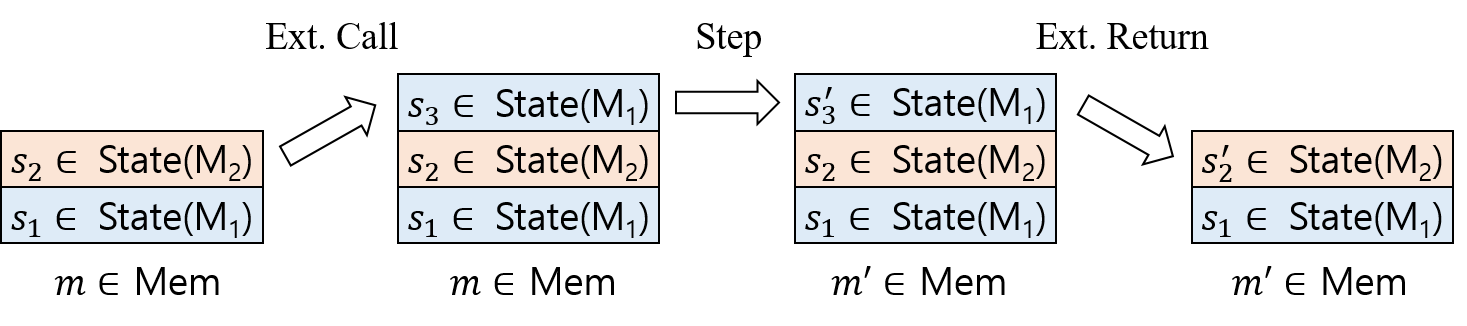
\includegraphics[width=0.9\linewidth]{images/intersem.png}
\caption{An execution of interaction semantics}
\label{fig:inter-sem}
\end{figure}

%% marshalling unmarshalling
%% marshalling the argument values into a list of values
%% setting the initial core states, unmarshalling the list of arguments.
%% at\_external: marshalling the argument values into a list of values
%% after\_external: unmarshalling the return value into
%% halted: marshalling the return value
%% corestep: use the underlying language semantics

Finally, note that the language semantics of C, assembly and
intermediate languages can be lifted to give a module semantics by
defining \texttt{corestep} to be the same as the execution step of the
language's semantics, and the other module operations to reflect the
calling conventions. Note also that all language-specific resources
(\ie other than the memory)
such as the register-file of assembly 
reside inside the module state, and thus are
duplicated at each invocation of a module.

%% One can lift a \cc{} language semantics into a core semantics by providing the interfaces:
%% Note that it is possible to define a core semantics using a mathematical specification.


\subsection{Open Simulation}
% \emph{core semantics}
The interaction semantics of \ccc{} gives a way to execute an
\emph{open} module $\module$ (\ie invoking external functions defined
outside $\module$) in isolation by providing a logical mechanism to
reflect possible interference from external function calls. More
specifically, the semantics provides two meta-level functions
$\mathtt{at\_external}$ and $\mathtt{after\_external}$. First,
$\mathtt{at\_external}~\stt = \mathtt{Some}~(f,\vec{v})$ denotes that
at language state $\stt$, an external function pointed to by a
function pointer $f$ is called with arguments $\vec{v}$. Second,
$\mathtt{after\_external}~r~\stt$ denotes the language state after the
external function call at $\stt$, assuming the call returned a value
$r$.
%% See \Cref{sec:overview-semantics:background} and \Cref{sec:main-semantics}
%% for more details about the interaction semantics.

%% $\mathtt{at\_external}$ detecting an external function call:
%% $\mathtt{at\_external}~\stt = \mathtt{Some}~(f,\vec{v})$ denotes that
%% at language state $\stt$, an external function pointed to by a
%% function pointer $f$ is called with arguments $\vec{v}$. Also, it
%% provides a meta-level function $\mathtt{after\_external}$ constructing the language state after
%% an external function call: $\mathtt{after\_external}~r~\stt$ denotes
%% the language state after the external function call at $\stt$, assuming
%% the call returned a value $r$. See \Cref{sec:main-semantics} for more details
%% about the interaction semantics.
%% \jeehoon{I don't think it's necessary to mention the word ``core semantics''. Why not just saying
%%   it's interaction semantics?}

Using interaction semantics, \ccc{} defines \emph{structured
  simulations} relating two open modules.
Here we briefly review the key ideas behind them,
which also occurred elsewhere, \eg in~\cite{pb,neis:pilsner,PLDI15}. \todo{check PLDI15}
First, unlike the closed simulations above,
structured simulations explicitly specify value and memory relations
(evolving over time) because values and memory are shared with external modules.
Specifically, such relations are defined using Kripke-style possible worlds,
called \emph{structured injections} \revision{(see \Cref{sec:overview-verification:injection} for more details)},
by giving $(i)$ a future world relation $\sqsupseteq$ for which
$w' \sqsupseteq w$ denotes that $w'$ is a future world of $w$;
and $(ii)$ value and memory relations at each world~$w$, denoted
$\mathtt{vrel}(w)$ and $\mathtt{mrel}(w)$.  Then, a
structured simulation $R$ gives a relation between machine
states at each world $w$, denoted $R(w)$, and should satisfy the
\emph{open} simulation property (simplified for presentation purposes) given in \Cref{fig:open-sim}.
\begin{figure}[t]
$
\begin{array}{@{}l@{}}
\texttt{ 1:}~\forall w,~ \forall (\memsrc,\memtgt)\in \mathtt{mrel}(w),~\forall \stsrc,\sttgt,~((\memsrc,\stsrc),(\memtgt,\sttgt))\in R(w)\implies{} \\[.5mm]
\texttt{ 2:}~\quad\textbf{match}~\mathtt{at\_external}~\stsrc~\textbf{with}\\[.5mm]
\texttt{ 3:}~\quad\mathtt{|}~\mathtt{Some}~(f_\src,\vec{v}_\src) \Rightarrow{}\\[1mm]
\texttt{ 4:}~\quad\quad \exists f_\tgt,\vec{v}_\tgt,~ \mathtt{at\_external}~\sttgt = \mathtt{Some}~(f_\tgt,\vec{v}_\tgt) \land{}\\[1mm]
\texttt{ 5:}~\quad\quad \fbox{$(f_\src,f_\tgt)\in \texttt{vrel}(w) \land (\vec{v}_\src,\vec{v}_\tgt) \in \overrightarrow{\texttt{vrel}(w)}$} \land{} \\[2mm]
\texttt{ 6:}~\quad\quad \dashbox{$\forall w' \sqsupseteq w,~\forall (\memsrc',\memtgt')\in\texttt{mrel}(w')$,}~ \dashbox{$\forall (r_\src,r_\tgt)\in \texttt{vrel}(w'),$}\\[2.5mm]
\texttt{ 7:}~\quad\quad ((\memsrc',\mathtt{after\_external}~r_\src~\stsrc),(\memtgt',\mathtt{after\_external}~r_\tgt~\sttgt))\in R(w') \\[.5mm]
\texttt{ 8:}~\quad\mathtt{|}~\mathtt{None} \Rightarrow{} \\[-.5mm]
\texttt{ 9:}~\quad\quad\forall e, \memsrc', \stsrc',~ (\memsrc, \stsrc) \estep{e} (\memsrc',\stsrc') \implies {}\\[.5mm]
\texttt{10:}~\quad\quad \exists \memtgt',\sttgt',~ (\memtgt,\sttgt) \estep{\tau}^{\raisebox{-1mm}{\scriptsize$\ast$}} \estep{e}\estep{\tau}^{\raisebox{-1mm}{\scriptsize$\ast$}} (\memtgt',\sttgt') \land{}\\[1mm]
\texttt{11:}~\quad\quad \fbox{$\exists w' \sqsupseteq w,~ (\memsrc',\memtgt') \in \mathrm{mrel}(w')$} \land {} \\[2.5mm]
\texttt{12:}~\quad\quad((\memsrc',\stsrc'), (\memtgt',\sttgt')) \in R(w')\\
\texttt{13:}~\quad\textbf{end}
\end{array}
$
\caption{Structured (or, open) simulations (simplified for presentation purposes)}
\label{fig:open-sim}
\end{figure}
% \jeehoon{In \texttt{at\_external} case, how about allowing the source to take silent steps?  Or
%   maybe we can remove silent steps also from the previous paragraph on CompCert's verification.}

Here the simulation involves rely-guarantee reasoning and is split
into two cases: one for interactions with external modules and the
other for internal steps (omitting two more cases for function start and end,
for presentation purposes). Specifically, given
any world $w$, related memories at $w$ and machine states related by
the simulation relation $R$ at $w$ (line~1), we check whether the
source state is invoking an external function or taking an internal
step (line~2). In the former case (line~3), the target state should
also be invoking an external function (line~4) and the invoked
functions and arguments should be related by the value relation at the
world~$w$ (line~5), which is a \fbox{guarantee condition} to the external modules.
Then we assume that the invoked external
functions proceed to a future world $w'$ yielding related memories and
related return values at $w'$ (line~6), which is a \dashbox{rely condition} from the external modules.
Under the assumption, the machine
states after the external calls should also be related by the
simulation relation $R$ at the future world $w'$ (line~7). In the
latter case (line~8), for any internal step from the source state
(line~9), there should be corresponding internal steps from the
target state (line~10).  Then the resulting memories after the steps
should be related at some future world $w'$ (line~11), which is a
\fbox{guarantee condition} to the external modules.  Finally, the
machine states after the steps should also be related by the
simulation relation $R$ at the future world $w'$ (line~12).

At high level, this simulation property specifies that internal
executions of the source and target modules should be related in
lockstep satisfying the guarantee conditions to the external modules,
assuming that the rely conditions from them hold after each external
function call.  Note that the rely and guarantee conditions on memory
(at lines 6 and 11) are matched and also those on values (at lines 5
and 6) will be matched if we include the omitted cases for function
start and end. This matching---in addition to the fact that the same
rely/guarantee conditions are used globally (\ie for verification of
every module)---is crucial for proving preservation of the simulation
property after linking modules because otherwise what one module
assumes about the other modules will not match with what the other
modules guarantee.

To use structured simulations for compiler verification, \ccc{} proves
the following three key properties, where we say a source module
$\module$ simulates a target module $\module'$ if there exists a
structured simulation that relates $\module$ and $\module'$:
\begin{itemize}
\item \textbf{(\emph{Vertical Compositionality})}
  If $\module$ simulates $\module'$, which simulates $\module''$,
  then $\module$ simulates~$\module''$.
\item \textbf{(\emph{Horizontal Compositionality})}
  If $\module_1$ and $\module_2$ simulate
     $\module'_1$ and $\module'_2$ respectively,
  then the linked source module  $\module_1 \llink \module_2$ simulates
  the linked target module $\module'_1 \llink \module'_2$.
\item \textbf{(\emph{Adequacy})}
  If $\module$ simulates $\module'$,
  then $\beh{\module} \supseteq \beh{\module'}$.
\end{itemize}






\subsection{Memory Relations of \cc{}}
\label{sec:overview-verification:injection:original}
%
\cc{}'s memory model consists of a finite set of blocks of finite size
and a pointer value (or, an address) is a pair $(b,o)$ of a block id $b$ and an offset $o$ inside it.
The memory identity imposes that the source and target memories are identical;
and the extension that the two memories contain identical block ids and
each target block extends the corresponding source block
with more space and any values in it at the end.

A memory injection injects a subset of the source blocks into target blocks
without overlap. More precisely, a (selected) whole source block is injected into a single target block
while allowing multiple source blocks to be injected into the same target block without overlap.
This injection map specifies the \emph{public} areas of the source and target memories and the correspondence between them.
In other words, the corresponding addresses by the injection map are treated as \emph{equivalent} (public) pointer values,
%% and therefore
so that at those corresponding addresses,
only equivalent%
\footnote{Technically speaking, \cc{} allow more undefined values in the source
  because it proves refinement rather than equivalence between the source and target programs.}
values (\ie equivalent non-pointer values or corresponding addresses) should be stored .
All the areas that are not on the injection map are considered as \emph{private} areas of the source and target memories.





\chapter{Theory of RUSC}
\label{chap:rusc}
\section{Problems with Open Simulation}
\label{sec:overview-verification:problems}
%% \myparagraph{Problems}
%
%   9051 /   2839 = 3.2 (id)
%  22124 /   8129 = 2.7 (ext)
%  23564 /   9128 = 2.6 (inj)
%
% Total
%  54739 /  20096 = 2.7  (pass)
% 152363 /  92029 = 1.65 (meta)
% 207102 / 112125 = 1.84 (whole)
%
%% Structured simulations of \ccc{} suffer from the problem that
%% verification using them is significantly more costly than that using
%% closed simulations of \cc{}: the Coq scripts for the verification of
%% all passes in \ccc{} is roughly \todo{2.7} times as large as that in
%% the original \cc{} in terms of lines of code~(LOC).
%% \jeehoon{How about reporting significant lines of code (SLOC)?}

As discussed in the introduction, verification using structured
simulations is significantly more costly than that using closed
simulations.  The reasons are twofold.

First, \revision{while closed simulations freely allow arbitrary memory relations---%
therefore \cc{} uses three different kinds of memory relations to simply proofs---%
%% ---thereby \cc{} uses three relations, \emph{memory identity, extension and injection}---
structured simulations only allow a single type of memory relations
called \emph{structured injections} due to horizontal compositionality.}
%
The reason is that, as discussed above,
%% in the background section,
allowing different memory relations would introduce
different rely/guarantee conditions
thereby breaking simulation after linking (\ie horizontal
compositionality) due to the mismatch between different rely/guarantee
conditions.
%% To see the reason, recall that, as we have seen in the
%% background section, the rely/guarantee conditions are determined by the
%% memory (and value) relations and the same rely/guarantee conditions
%% should be used globally to preserve simulations after linking
%% modules (\ie to prove horizontal compositionality).
%% Therefore allowing different memory relations for verifying
%% different modules would be problematic for proving horizontal
%% compositionality together with adequacy.

\revision{Second,
%% the notion of structured injection of \ccc{} is more complex than that of
%% \emph{memory injection} of \cc{} and, as far as we understand, such
%% complexity is needed for vertical compositionality.
%% It is well known that
proving vertical compositionality for \emph{open} simulations is in general
very technical and involved~\cite{ICFP19,neis:pilsner}. Indeed the
proof for structured simulations is about 5,000 SLOC in Coq.
Moreover, vertical compositionality also introduces unnecessary complexities
in structured simulations of \ccc{} such as \emph{effect annotations}
and \emph{closedness under restriction} \cite{stewart:ccc}.}
%% which makes correctness proofs of compiler passes more involved
%% (see \Cref{sec:overview-verification:injection} for discussion).}

To sum up, although it is quite straightforward to prove horizontal
compositionality and adequacy for a single relation (\ie with the same
rely/guarantee conditions), it is challenging to prove $(i)$ vertical
compositionality even for a single relation and $(ii)$ horizontal
compositionality between different relations (\ie with different
rely/guarantee conditions).

%\section{Refinement Under Self-related Contexts (RUSC)}
\section{RUSC}
\label{sec:overview-verification:solution}

%% \myparagraph{Our Solution at High Level}
%
Our solution is twofold. First, we develop a general and abstract
theory, called \emph{Refinement Under Self-related Contexts (RUSC)},
which is inspired by the standard notion of contextual refinement
\revision{and the notion of self-related context from \cite{stewart:ccc}
  (see \Cref{sec:related} for comparison).}
%\scc{}~\cite{?} (see \Sref{sec:related} for comparison).
Specifically, given a set of (arbitrary and independent)
relations each of which is horizontally compositional and adequate,
RUSC completes the relations by giving a super-relation (\ie
including all of them) that is horizontally and vertically
compositional and also adequate. Second, we prove that
our version of structured simulations, called \emph{open simulations},
with almost arbitrary memory relations
are horizontally compositional and adequate,
so that we can apply RUSC to open simulations with any chosen set of memory relations.

\myparagraph{Theory of RUSC}
%
RUSC can be defined abstractly for any linking algebra, which consists
of a set of modules, $\Module$, with a notion of behavior\footnote{Behaviors just need to be defined for closed programs.
  Technically, we can give undefined behavior (UB) to open modules.
%  For open modules, invoking an unknown function can be defined as undefined behavior (UB).
}, denoted
$\beh{p}$ for $p\in\Module$, a linking operation~$\llink$ between modules
that is associative%
\footnote{\revision{Commutativity does not hold for linking of \cc{} modules
    because changes in the order of global variables affect the initial memory after loading
    due to \cc{}'s deterministic memory allocation.}},
\revision{and the identity (\ie empty) module $\identity \in \Module$}:
\[
\begin{array}{c}
\llink: \Module \times \Module \rightarrow \Module \\
\forall p,q,r\in\Module,~p \llink (q \llink r) = (p \llink q) \llink r \\
\revision{\forall p \in\Module,~ \identity \llink p = p \llink \identity = p} \\
\end{array}
\]
Note that RUSC can be applied to interaction semantics because it
allows linking between arbitrary modules sharing the same notions
of value and memory (see \Cref{sec:overview-semantics:background} and \Cref{sec:main-semantics} for details).

To define RUSC, let $\rels$ be a set of module relations each of which is horizontally
compositional and adequate: for any $R \in \rels$ and $p,p',q,q'\in \Module$,
\[
\begin{array}{r@{}l@{\qquad}l}
(p,p'),(q,q')\in R &{}\implies (p \llink q, p' \llink q') \in R &\textrm{(\emph{HorComp})} \\
(p,p') \in R &{}\implies \beh{p} \supseteq \beh{p'} &\textrm{(\emph{Adequacy})} \\
\end{array}
\]
Then the RUSC relation for $\rels$, denoted $\rusc_{\rels}$, is defined as follows:
\[
\begin{array}{rcl}
p \rusc_{\rels} p' &\text{\emph{iff}}& \revision{\forall c_1, c_2 \in \self{\rels},~
\beh{c_{1} \llink p  \llink c_2} \supseteq \beh{c_{1} \llink p' \llink c_2}} \\
\self{\rels} & \defeq & \setof{ c \in \Module \suchthat \forall R \in \rels,~ (c,c) \in R }
\end{array}
\]
The definition is simple: $p$ is RUSC-related to $p'$ if the behaviors of $p'$ refine those of $p$ under
arbitrary contexts that are related to themselves by every relation in $\rels$.
% \jeehoon{From the definition of $p \rusc_{\rels} p'$, I think maybe it's easier to distinguish the
%   module type and the list-of-modules type... I know it's vague. Let's discuss offline.}

\begin{theorem}[Properties of RUSC]\label{thm:rusc} The RUSC relation $\rusc_\rels$ satisfies the following key properties.\\[.5mm]
$
\begin{array}{@{\quad}lrl}
 \text{(Inclusion)} &\forall R \in \rels,& R \subseteq {\rusc_\rels} \\[.5mm]
 \text{(Adequacy)} &\forall p,p'\in\Module,& p \rusc_{\rels} p' \implies \beh{p} \supseteq \beh{p'} \\[.5mm]
 \text{(VerComp)} &\forall p,p',p''\in\Module,& p \rusc_{\rels} p' \land p' \rusc_{\rels} p'' \implies p \rusc_{\rels} p'' \\[.5mm]
 \text{(HorComp)} &\forall p,p',q,q'\in \self{\rels},&   p \rusc_{\rels} p' \land  q \rusc_{\rels} q' \implies p \llink q \rusc_{\rels} p' \llink q' \\[.5mm]
 \revision{\text{(SelfComp)}} & \revision{\forall p,q \in \self{\rels},}& \revision{p \llink q \in \self{\rels}}
\end{array}
$
\end{theorem}
Note that horizontal compositionality holds only for self-related
modules, which, however, is not a big deal in practice as we will
discuss below.
\begin{proof}
The proof of the theorem is simple.  The
inclusion $R \subseteq {\rusc_\rels}$ trivially follows from the
horizontal compositionality and adequacy of $R$.  Adequacy of
$\rusc_\rels$ directly follows from the definition of $\rusc_\rels$ by
taking the empty context. Vertical compositionality (\ie transitivity)
of $\rusc_\rels$ holds trivially by definition.  Horizontal
compositionality, $p \llink q \rusc_{\rels} p' \llink q'$, is proven
in two steps using transitivity: $(i)$ $p \llink q \rusc_{\rels} p' \llink q$,
which follows from the definition of $p \rusc_{\rels} p'$ since $q\in\self{\rels}$,
and $(ii)$ $p' \llink q \rusc_{\rels} p' \llink q'$, which follows
similarly since $q \rusc_{\rels} q'$ and $p'\in\self{\rels}$.
%% ${R} \subseteq {\rusc_{\setofz{R}}}$ and
%% ${\rels} \subseteq {\rels'} \implies {\rusc_{\rels}} \subseteq {\rusc_{\rels'}}$
\revision{Finally, self-relatedness is closed under composition
because every relation in $\rels$ is horizontally compositional.}
\end{proof}

The reason why vertical compositionality is easily proven for RUSC
is that we essentially prove it for \emph{closed} programs by
closing an open module with contexts. Indeed, the technical
difficulties with vertical compositionality for open
simulations arise from the openness: it is difficult to set up a
setting properly with arbitrary future memories given after an external
function call.

The reason why horizontal compositionality holds between different
relations is interesting. Directly composing two simulations $(p,p') \in R_1$
and $(q,q') \in R_2$ with different relations $R_1$ and $R_2$
does not work in general. However, each simulation can be easily
extended with identical contexts because a pair of identical modules
usually respects any sensible relational principles. Therefore,
we have $(p \llink q ,p' \llink q) \in R_1$ and
$(p' \llink q ,p' \llink q') \in R_2$, which can be transitively composed
by vertical compositionality just as discussed above.
%% \jeehoon{I think we can say our horizontal compositionality proof, not the entire RUSC, is inspired
%%   from \scc{}.}

To sum up, RUSC provides a general condition for composing
different relational proofs: each proof just needs to be compatible
with its context modules in terms of self-relatedness, not necessarily
with their relational proofs.
%% instead of their relational proofs.

%% \begin{figure}
%%   \centering
%%   \includegraphics[width=0.70\linewidth]{rusc.jpg}
%%   \caption{Proving compositional compiler correctness with RUSC
%%   }
%%   \label{fig:rusc}
%% \end{figure}

%% \todo{add a fig:
%%   small horizontal compositionality figure,
%%   say that compatibility of rely/guarantee conditions between two relations (no)
%%   say that compatibility of rely/guarantee condition vs. the context I linked with. (yes)
%% }

\myparagraph{Open Simulations}
%
%% \todo{talk about analysis}
%% Since we can obtain vertical and horizontal compositionality
%% using RUSC, we can use simpler simulation relations (with different
%% memory relations)---which we call \emph{open simulations}---than
%% structured simulations (with structured injections).
%% Basically, open simulations contain only the core mechanism of
%% structured simulation presented in \Cref{sec:overview-verification:background}
%% without unnecessary complications needed to prove vertical
%% compositionality.

\revision{Since we can obtain vertical and horizontal compositionality using RUSC,
we can use open simulations with almost arbitrary memory relations.}
More specifically, we prove that open simulations with
\emph{any} Kripke-style memory/value relation satisfying certain minimal
conditions (see \Cref{sec:main-verification:parameter} for details) are horizontally compositional
and adequate. Since the required conditions are so minimal, they are
satisfied by the three memory relations---memory identity, extension
and injection---and also by a more powerful relation,
called \emph{memory injection with module-local invariants}.
This new memory relation is needed to
verify a new pass we added, called \texttt{Unreadglob}, which
requires reasoning about module-local states enabled by \emph{static}
variables of C (see \Cref{sec:overview-modulelocal} for details).

%% (emphasize that RUSC allows different techniques for different passes.
%% Additionally, analysis passes and assumptions on global variables).
Note that unlike \cc{} 2.1 on which \ccc{} is based, \cc{} 3.5
implements a static analyzer performing value analysis, which is used by
several passes. In order to support independent modular verification of such analyzers,
we also parameterize open simulations with memory predicates---representing the
analysis results of such analyzers---and
prove their horizontal compositionality and adequacy (See \Cref{sec:main-verification} for details).

\myparagraph{Applications} In our paper, we use RUSC
% with open simulations
in two situations: compiler and program verification.
%% \jeehoon{On paragraph name: how about ``Applications''?  It sounds more general.}

First, we give an abstract example for compiler
verification.  Suppose our source program is written in three modules,
\texttt{a.c}, \texttt{b.c} and \texttt{c.asm}, and compiled via
multiple passes: $\texttt{a.c}\to\texttt{a.il1}\to\texttt{a.asm}$ and
$\texttt{b.c}\to\texttt{b.il2}\to\texttt{b.il3}\to\texttt{b.asm}$,
each of which is verified using a different relation as follows:
\[
\begin{array}{l}
  (\texttt{a.c},\texttt{a.il1}) \in R_1 \quad (\texttt{a.il1},\texttt{a.asm}) \in R_2 \\
  (\texttt{b.c},\texttt{b.il2}) \in R_3 \quad
  (\texttt{b.il2},\texttt{b.il3}) \in R_4 \quad
  (\texttt{b.il3},\texttt{b.asm}) \in R_5
\end{array}
\]
%
Then as long as the \emph{end modules}, \texttt{a.c}, \texttt{b.c}, \texttt{a.asm},
\texttt{b.asm}, \texttt{c.asm}, are self-related by the relations $R_1,\ldots,R_5$,
using RUSC we can obtain the following behavioral refinement:
\[
\beh{\texttt{a.c} \llink \texttt{b.c} \llink \texttt{c.asm}} \supseteq \beh{\texttt{a.asm} \llink \texttt{b.asm} \llink \texttt{c.asm}}
\]
The underlying reasoning is simple: for $\rels=\setof{R_1,\ldots,R_5}$, we get
\begin{itemize}
\item $\texttt{a.c} \rusc_\rels \texttt{a.asm}$ and $\texttt{b.c} \rusc_\rels \texttt{b.asm}$
  by Inclusion and VerComp of \Cref{thm:rusc};
\item $\texttt{c.asm} \rusc_\rels \texttt{c.asm}$ since
  %% $\texttt{c.asm} \in \self{\rels}$ and thus
  $(\texttt{c.asm},\texttt{c.asm}) \in R_1 \subseteq \rusc_\rels$
  by Inclusion of \Cref{thm:rusc};
  %% \jeehoon{I don't understand it..}
\item $\texttt{a.c} \llink \texttt{b.c} \llink \texttt{c.asm} \rusc_\rels \texttt{a.asm} \llink \texttt{b.asm} \llink \texttt{c.asm}$
  by HorComp of \Cref{thm:rusc};
\item $\beh{\texttt{a.c} \llink \texttt{b.c} \llink \texttt{c.asm}} \supseteq \beh{\texttt{a.asm} \llink \texttt{b.asm} \llink \texttt{c.asm}}$ by Adequacy of \Cref{thm:rusc}.
\end{itemize}
Note that we need to prove the self-relatedness only for the end
modules because we only link those, not the intermediate ones
like \texttt{a.il1}, \texttt{b.il2}, \texttt{c.il3}.
Moreover, proving self-relatedness by a relation is typically
straightforward as long as the relation is sensibly defined.  Indeed,
we could easily prove that \emph{all} Clight\footnote{Clight is taken
  as the source language in most verification projects using \cc{}
  such as VST~\cite{VST}, CertiKOS and even \ccc{}.
  However, we also prove behavioral refinement w.r.t. the C source language
  (see \Cref{sec:results}).
}
and assembly programs are
self-related by all the relations used by \ccm{}
(\ie open simulations with memory identity, extension,
and injection with or without module-local invariants).
%% \jeehoon{How about ``we could easily prove that \emph{all} C, Clight, ...''}

Second, we demonstrate, via small but interesting examples (see \Cref{sec:overview-modulelocal}),
% (see \Cref{sec:overview-modulelocal} and \Cref{sec:utod-verification}),
%% the possibility
that our framework can be used to verify program modules
against (open) mathematical specification modules, written in Coq's Gallina language.
In the above example, for instance, we can prove
\[
\begin{array}{c}
\texttt{a.spec} \rusc_\rels \texttt{a.c}\quad
\texttt{b.spec} \rusc_\rels \texttt{b.c}\quad
\texttt{c.spec} \rusc_\rels \texttt{c.asm}
\\
\texttt{abc.spec} \rusc_\rels \texttt{a.spec} \llink \texttt{b.spec} \llink \texttt{c.spec}
\end{array}
\]
and link them together with the compiler correctness results above to get
\[
\beh{\texttt{abc.spec}}
\supseteq %% \rusc_\rels
%% \texttt{a.spec} \llink \texttt{b.spec} \llink \texttt{c.spec}
%% \rusc_\rels
\beh{\texttt{a.asm} \llink \texttt{b.asm} \llink \texttt{c.asm}}
\]
as long as the mathematical specification modules \texttt{a.spec},
\texttt{b.spec}, \texttt{c.spec}, \texttt{abc.spec} are in $\self{\rels}$,
which is usually straightforward to prove.

\myparagraph{Comparison to Contextual Refinement}
%
As one can easily see, RUSC refines the standard notion of contextual
refinement: instead of quantifying over \emph{all} contexts, RUSC
quantifies over only \emph{self-related} contexts. The main difference
is that RUSC gives the notion of well-behaved context w.r.t. a given
set of program relations (\ie reasoning principles) in terms of
contexts self-related by them.  This is particularly useful when not
all contexts are well behaved.  For example, in the interaction
semantics allowing mathematical specification modules as above, one can
easily write a specification module that arbitrarily changes the whole
memory including other modules' private memory. Under the presence of
such ill-behaved contexts, the contextual refinement will end up being too
strong preventing any reasoning about private memory such as
functions' stack frames. On the other hand, RUSC w.r.t. a set of
sensible relations will rule out such bad contexts and give us a sensible (better) relation.
%% even in the presence of such ill-behaved contexts.

%% \todo{Revise:
%% To sum up, the theory of RUSC tells that different relational proofs
%% well compose as long as the contexts of your interest are self-related
%% by the proof techniques of your interest.
%% }

%% because RUSC quantifies over only well-behaved contexts (\ie self-related ones
%% w.r.t. the given set of relations).

%% \hide{
%% We first review \cc{}'s correctness statement and its verification
%% method (\Cef{sec:background:cc}), and then how \ccc{} extends \cc{}
%% to allow multi-language programs (\ie programs composed of modules written in
%% different languages including C, assembly and \cc{}'s intermediate languages) (\Cref{sec:background:ccc}).
%% %% \ccc{} generalizes them to handle interactions between modules written in different
%% %% languages (\Cref{sec:background:ccc}).
%% In addition, we review key semantic techniques used for verification of CompCert.
%% %% called undefined behavior and logical memory
%% (\Cref{sec:background:ub}).
%% }




%%% Local Variables:
%%% mode: latex
%%% TeX-master: "main"
%%% End:


\chapter{Application: CompCertM}
\label{chap:compiler}
%% \chapter{\;\;\;\;Compiler Verification: CompCertM} %%이러면 (toc 말고 본문에서) 넘침
\chapter{\;\;\;\;Compiler Verification}
\label{sec:compiler}

\section{Background}
\label{sec:compiler:background}

\subsection{A Brief Introduction on CompCert}

\myparagraph{Undefined Behavior}



\section{Problems}
\label{sec:compiler:problems}

The problems with the interaction semantics of \ccc{} are that it does
not satisfy two adequacy properties. First, the adequacy w.r.t. C says
that for any C modules $M_1,\ldots,M_n$, the behaviors of the linked
program according to interaction semantics $\beh{M_1 \llink
  \ldots \llink M_n}$ should \emph{be included in} those according to the
physical semantics $\beh{M_1 \plink \ldots\plink M_n}$.  The reason for
failure was quite simple and we could easily fix it: unlike \ccc{}, we allow passing
the \texttt{undef} value to an external module since the C semantics
does so, while we turn ill-typed values into \texttt{undef} when they
are passed to an external module.

Second, the failure of the adequacy w.r.t. assembly is more serious.
Adequacy says that for any assembly modules $M_1,\ldots,M_n$,
the behaviors of the linked program according to interaction
semantics $\beh{M_1 \llink \ldots \llink M_n}$ should \emph{include}
those according to the physical semantics $\beh{M_1 \plink \ldots\plink M_n}$.
Note that the direction is opposite since assembly is the target language.
As discussed before, the reason for failure is that
the interaction semantics of \ccc{} does not have a mechanism to detect
illegal interference and make it undefined behavior~(UB).

\section{Solution}
\label{sec:compiler:solution}

We identify the sources of inadequacy w.r.t. assembly as violations of
three assumptions made by standard compilers: two on the registers and one on the stack.
We discuss why they 
cause problems with counterexamples and show how to semantically
handle them without changing the underlying language semantics.

\subsection{Assumptions on the Registers}
\label{sec:overview-semantics-register}
%
The two problematic assumptions on the registers are that
an invoked assembly function $(i)$ should
preserve the initial values of the callee-save registers, and $(ii)$
should not access the memory via the leftover pointer values remaining
in those registers that are not involved in passing meaningful information to the callee,
which we henceforth call \emph{\nip{}} registers.
%% in those registers, which we call \emph{non-passing} registers,
%% that are not involved in passing information to the callee.
%% the \emph{non-passing} registers (\ie those registers not involved
%% in passing information to the callee).
%% We discuss these two conventions together because it is nontrivial to find a
%% single model that enforces both conventions at the same time.
%% \jeehoon{I don't understand the last sentence..}
%% \jeehoon{``\nip{}'': how about ``opaque''?}

\begin{figure}[t]
\fbox{\begin{minipage}{.9pc}\mbox{}\\[15.25mm](a)\\[13.45mm]\mbox{}\end{minipage}}
\hspace*{-2.7mm}
\begin{minipage}{0.70\textwidth}
\begin{Verbatim}[frame=single]
int main()   {          main:
  int* x = malloc(8);     ...
  x[0] = 0;               *(%rbx) = 0;
  x[1] = 1;               *(%rbx + 4) = 1;
  f();               -->  f();
  out(x[0]);              out(*(%rbx));
  ...                     ...
}
\end{Verbatim}
\end{minipage}
$\mbox{}~\mathlarger{\mathlarger{\mathlarger{\mathlarger{\mathlarger{\llink}}}}}~\mbox{}$
\\
\vspace{3mm}
\\
\fbox{\begin{minipage}{.9pc}\mbox{}\\[10.50mm](b)\\[8.70mm]\mbox{}\end{minipage}}
\hspace*{-2.7mm}
\begin{minipage}{0.33\textwidth}
\begin{Verbatim}[frame=single]
f:
  if (g(%rbx))
    %rbx = %rbx + 4;
  else
    *(%rbx) = 1;

\end{Verbatim}
\end{minipage}
\caption{A counterexample showing the problem with the assumptions on the registers}
\label{fig:reg-convention}
\end{figure}

\myparagraph{Counterexamples}
%
The example in \Cref{fig:reg-convention} shows how violations of the two
assumptions can invalidate correct compiler translations.
%% \jeehoon{I think counterexample should go to the problems section.}
%
The code in the left box~(a) shows a standard translation of C code into assembly
(written in pseudocode) performed by mainstream compilers like GCC and LLVM, where the accesses to
the array \texttt{x} are translated into accesses via the register
\texttt{\%rbx} assuming that \texttt{\%rbx} is set to contain the
address of \texttt{x}. An important point here is that the compiler
assumes that $(i)$ the value of \texttt{\%rbx} is unchanged across
the function call \texttt{f()} since it is a callee-save register,
and also $(ii)$ the values in the array pointed to by \texttt{\%rbx} are
unchanged across \texttt{f()} since the array's addresses do not escape
except via \nip{} registers like \texttt{\%rbx}.
Therefore, the compiler expects that \texttt{out(*(\%rbx))} in the target code
correctly outputs \texttt{0}.

The right box~(b) presents an example of handwritten assembly
(written in pseudocode) for function \texttt{f} that violates the
above two assumptions of the compiler. The code either increments
\texttt{\%rbx} by \texttt{4} or writes \texttt{1} to \texttt{*(\%rbx)}
depending on the result of call to \texttt{g}.  Now if we link the assembly
code in (a) and that in (b) together, one can easily see that
\texttt{out(*(\%rbx))} incorrectly outputs~\texttt{1} instead
of \texttt{0} in either case: in the former case, \texttt{\%rbx}
points to the second element of the array~\texttt{x}, which contains
\texttt{1}; in the latter case, the value of \texttt{*(\%rbx)} is
directly updated to \texttt{1}. Therefore, it makes sense to
define those illegal behaviors of (b) as undefined behavior~(UB).

\myparagraph{Our Model}
\label{sec:compiler:solution:model}
%
We present our model making the illegal behaviors UBs
in stages, explaining at each stage why naive models do not work.
%% \jeehoon{What's the difference between ``stage'' and ``state''?}
%% \jeehoon{We have ``Our Solution'' paragraph inside ``Our Solution'' section. How about moving
%%   counterexample to the problems section, and giving a paragraph to each stage?}

First, in order to enforce the preservation of callee-save register
values, we store the initial values of the callee-save registers at
the \texttt{init-core} step of assembly modules; and check, at the
\texttt{halted} step, whether the final values of those registers are
equal to the stored initial values and if not, raise UB.  Here, the
question is, when a new core with a fresh register file is pushed into the core stack,
what values should be set as initial values of the \nip{}
registers including all of the callee-save registers.  Since the
registers may contain arbitrary values in the physical assembly
semantics, a natural choice would be to initially set them to contain
the \texttt{undef} value, which is an abstract value representing all
possible values. Indeed, this is the choice of \ccc{}.  However, there
is a serious problem. Since, for instance, \texttt{undef + 4} results
in \texttt{undef}, checking whether the final values of callee-save
registers are equal to the initial values, \ie \texttt{undef}, is
not sufficient. Specifically, the assembly code in (b) above
does not raise UB in this new semantics in case \texttt{g(\%rbx)} returns \texttt{1}
because the initial and final values of \texttt{\%rbx}
are both \texttt{undef} and thus equal
even though the callee-save register \texttt{\%rbx} is incremented
by \texttt{4} in the physical semantics.

Second, another natural solution would be to initially set the
\nip{} registers to nondeterministically contain arbitrary
values including \texttt{undef}. Though this model is more flexible,
it still has a problem. For instance, in the above example, to
simulate the physical behaviors of the assembly function \texttt{f} in
interaction semantics, one can set the initial value of \texttt{\%rbx} to
be either $(i)$ \texttt{undef} (\ie a more abstract value than the physical one), or
$(ii)$ a pointer to the array \texttt{x} (\ie a value equivalent to the physical one):
other values cannot be used since they are not refined by the value of \texttt{\%rbx} in the target,
which is required since the value is passed to an unknown function~\texttt{g}.
In the former case, if
\texttt{g(\%rbx)} returns \texttt{1}, we have the same problem with
callee-save checking as shown above.  In the latter case, if
\texttt{g(\%rbx)} returns \texttt{0}, the function \texttt{f}
successfully updates the array~\texttt{x} thereby invaliding the
translation in (a) as illustrated above.

We solve this problem by further revising the second model:
nondeterministically allocating an arbitrary number of \emph{junk
  blocks} (\ie blocks of size zero) and then initializing the
\nip{} registers with arbitrary non-pointer values or
\emph{junk pointers} (\ie pointers to the junk blocks).  Then we can
simulate the physical behaviors by initializing each register $r$
$(i)$ with the same non-pointer value if the physical value of $r$ is
a non-pointer value; and $(ii)$ otherwise with a fresh junk pointer.
The high-level idea is that, like \texttt{undef}, a junk pointer is
more abstract (\ie causing more UBs) than any pointer but, unlike
\texttt{undef}, sufficiently distinguishable. For instance,
in the previous example, if \texttt{g(\%rbx)} returns \texttt{1},
the initial and final values of \texttt{\%rbx} (\ie $p$ and $p+4$ for a junk pointer $p$)
are distinguished thereby raising UB by the callee-save checking;
if \texttt{g(\%rbx)} returns \texttt{0},
the memory access \texttt{*(\%rbx) = 1} raises UB because \texttt{\%rbx}
points to a junk block of size zero.

Finally, note that introducing nondeterminism as above is not a
showstopper thanks to the mixed simulation, as discussed in
\Cref{sec:overview-verification:mixedsim}: we can do forward
simulation everywhere except for the \texttt{init\_core} step of
assembly modules, where we should do backward simulation.

\subsection{Assumptions on the Stack}
\label{sec:overview-semantics-memory}
%
The problematic assumption on the stack is that the
\emph{outgoing arguments area} of a caller's stack (\ie where overflowing function
arguments are stored) should be fully \emph{owned} by the callee. In
other words, the callee can assume that the arguments area is never
modified by others unless its addresses are revealed to the public by
the callee itself.

\begin{figure}[t]
\fbox{\begin{minipage}{.9pc}\mbox{}\\[10.45mm](a)\\[8.65mm]\mbox{}\end{minipage}}
\hspace*{-1.9mm}
\begin{minipage}{0.255\textwidth}
  \begin{Verbatim}[frame=single]
main:
  ...  
  leak = %rsp;
  f(..., 0);
g:
  *leak = 1;
  \end{Verbatim}
\end{minipage}
$\mbox{}~\mathlarger{\mathlarger{\mathlarger{\mathlarger{\mathlarger{\llink}}}}}~\mbox{}$
\fbox{\begin{minipage}{.9pc}\mbox{}\\[10.45mm](b)\\[8.65mm]\mbox{}\end{minipage}}
\hspace*{-1.9mm}
\begin{minipage}{0.695\textwidth}
  \begin{Verbatim}[frame=single]
void f(..., int64_t x)       f:
{                              ...
  out(x);                      out(*(%rax));
  g();                  -->    g();
  out(x);                      out(*(%rax));
}                              ...
  \end{Verbatim}
\end{minipage}
\\[1mm]
\fbox{\begin{minipage}{.9pc}\mbox{}\\[15.90mm](c)\\[15.10mm]\mbox{}\end{minipage}}
\hspace*{-2.7mm}
\begin{minipage}{.95\textwidth}
\fbox{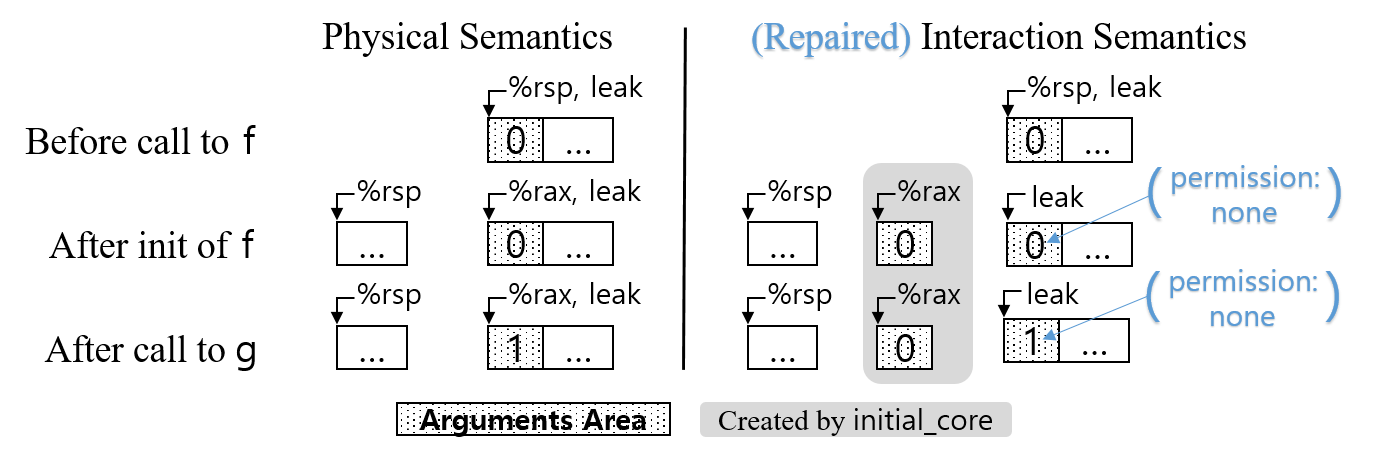
\includegraphics[width=.983\textwidth]{images/ex-stack.png}}
\end{minipage}
%% \fbox{\begin{minipage}{.8pc}\mbox{}\\[4.53mm](c)\\[3.73mm]\mbox{}\end{minipage}}
%% \hspace*{-1.9mm}
%% \begin{minipage}{.95\textwidth}
%%   \begin{Verbatim}[frame=single]
%%                      Physical Semantics         Interaction Semantics
%%                             %rsp           |                  %rsp       
%% Before call to f:           [=0=| ... ]    |                  [=0=| ... ]
%%                     %rsp    %rax           |    %rsp    %rax             
%%  After init of f:   [ ... ] [=0=| ... ]    |    [ ... ] [=0=] [=0=| ... ]
%%                     %rsp    %rax           |    %rsp    %rax             
%%  After call to g:   [ ... ] [=1=| ... ]    |    [ ... ] [=0=] [=1=| ... ]
%%   \end{Verbatim}
%% \end{minipage}
\caption{A counterexample showing the problem with the assumption on the stack}
\label{fig:stack-convention}
\end{figure}

\myparagraph{Counterexamples}
%
The example in \Cref{fig:stack-convention} shows how violations of the assumption
can invalidate correct compiler translations.
%
The box~(a) shows handwritten assembly code implementing two functions
\texttt{main} and \texttt{g}; the box~(b) shows a standard translation
of C code into assembly essentially performed by \texttt{gcc -O0}; and
the left-hand side (LHS) of the box~(c) depicts the shape of the stack
during execution in the physical semantics.
The function \texttt{main} stores the address of the
outgoing arguments area (\ie \texttt{\%rsp} as depicted in LHS of (c))
in the global variable \texttt{leak} and invokes the function
\texttt{f}, where the last argument \texttt{0} is stored in the
arguments area of the stack. Then the function \texttt{f} makes three
function calls, \texttt{out(x)}, \texttt{g()} and \texttt{out(x)},
where the argument \texttt{x} is directly read from the arguments area
pointed to by \texttt{\%rax} in the assembly, as depicted in LHS of
(c), and \texttt{out(x)} outputs the read value.  Finally, the
function \texttt{g} updates the arguments area pointed to by
\texttt{leak} with~\texttt{1}, as depicted in LHS of (c), between the
two function calls \texttt{out(x)}.

An important point here is that the compiler assumes that the
arguments area (\ie \texttt{\%rax}) is unchanged across the
function call \texttt{g()} since it is fully owned by \texttt{f}.
Therefore, the compiler expects that both calls
\texttt{out(*(\%rax))} in the target code correctly output
\texttt{0}. However, since the function \texttt{g} updates the
arguments area with \texttt{1} via \texttt{leak}, the two calls
incorrectly output \texttt{0} and~\texttt{1}.
We confirmed this incorrectness by
compiling \texttt{f} with \texttt{gcc -O2}, which
eliminates the second load \texttt{*(\%rax)} by propagating
the result of the first load across \texttt{g()}
thereby outputting \texttt{0} twice.

\myparagraph{Our Model}
%
In order to solve the problem, we have to distinguish accesses to the
arguments area via the caller from those via the callee and define the
former as UB. Though making such distinction is difficult in the
physical semantics, fortunately it is already made in interaction
semantics due to the language-independent design. For example, consider
the interaction semantics of the above example, depicted in the
right-hand-side (RHS) of \Cref{fig:stack-convention}~(c).  The
difference is that when the assembly function \texttt{f} is invoked,
the initialization process (\ie \texttt{init\_core}) of the module
semantics newly constructs the arguments area of the stack from the
given logical arguments in order to make an environment needed to
execute the assembly function \texttt{f}. This is essentially needed
because the caller may not be an assembly module so that it may not
have its own stack at all.  Then the callee sees the new arguments
area created by \texttt{init\_core} while the caller (in assembly)
sees the original arguments area.

Although the original interaction semantics does not prevent access to
the arguments area via the caller, we can easily fix it.
%% Now we can easily repair the original interaction semantics to make
%% those accesses to the arguments area via the caller as UB during the
%% lifetime of the callee.
We simply $(i)$ turn off the access
permission of the original arguments area in the \texttt{at\_external}
step of the caller module, and $(ii)$ turn it back on in the
\texttt{after\_external} step. Note that the notion of permission
%% is already an existing feature of
already exists in the \cc{} semantics, so that we do not
need to strengthen it. In the above example again,
the update by \texttt{g} will raise UB since the original argument area pointed
to by \texttt{leak} has no access permission.


\subsection{Mixed Simulation}
\label{sec:overview-verification:mixedsim}

While the target language of \cc{} is deterministic (more precisely,
the source is receptive and the target is determinate) thereby mostly
using forward simulations, the repaired interaction semantics of
\ccm{} is inherently nondeterministic to handle illegal interference from assembly modules
%% enforce the assembly calling conventions
(\Cref{sec:compiler:solution:model}) thus preventing the
use of forward simulation.
%% While it is theoretically possible to convert the \cc{}
%% verification from forward to backward simulations, it would incur a
%% significant cost since a compiler pass typically compiles a single
%% instruction in the source down to several instructions in the target.
%% %% due to the nature of source and target languages and the size of verification.
%% For this reason, determinism
%% has been considered ``instrumental for the simulation proofs of the compiler passes and its absence
%% is a show stopper''~\cite{besson:intptr}.
% Extending \cc{}'s semantics with such nondeterministic features can potentially cause significant
% overhead, as it invalidates forward simulation and enforces one to use backward simulation, which
% effectively means one should re-establish simulation proof from the scratch.  In literature, it is
% even said that

In order to recover the ability to use forward simulation in the occasional presence of nondeterminism,
we adopt the idea of \emph{mixed (forward-backward) simulation} from \cite{neis:pilsner}.
%% To embrace nondeterminism with low verification cost, we develop more general simulations, called
%% \emph{mixed simulations}, that (mostly) allow forward reasoning in the (occasional) presence of
%% nondeterminism.
The key observation is that
the requirement for using forward simulations (\ie determinism of the target) is a per-state property,
not a per-language property: as long as a particular target machine state is \emph{locally deterministic} (\ie its next state is unique),
one can do forward simulation at that state.
%% conversion from backward to forward simulations
%% requires only the current target \emph{machine state}, not the entire target \emph{language}, to be
%% deterministic.
Based on this observation, mixed simulations selectively allow forward
simulation when the target is locally deterministic, in addition to
the default backward simulation.
%% for each pair of related machine states, we allow the verifier to
%% \emph{choose} to perform either forward or backward reasoning, requiring that forward reasoning is
%% used only for locally deterministic target machine states.
%
Specifically, we say that a relation $R$ is a (closed) mixed simulation if
for all $(\mssrc, \mstgt) \in R$,
%% \makebox[\linewidth]{\makebox[1.2\linewidth]{
%% \begin{minipage}{1.2\linewidth}
\begin{enumerate}
\item
  $\forall e, \mstgt',~ \mstgt \estep{e} \mstgt' \implies {} $ \\
  $ \exists \mssrc',~ \mssrc \estep{\tau}^{\raisebox{-1mm}{\scriptsize$\ast$}} \estep{e}\estep{\tau}^{\raisebox{-1mm}{\scriptsize$\ast$}} \mssrc' \land (\mssrc', \mstgt') \in R$; or
\item
  $\forall e, \mssrc',~ \mssrc \estep{e} \mssrc' \implies {} $ \\
  $ \exists \mstgt',~ \mstgt \eustep{\tau}^{\raisebox{-1mm}{\scriptsize$\ast$}} \eustep{e}\eustep{\tau}^{\raisebox{-1mm}{\scriptsize$\ast$}} \mstgt' \land (\mssrc', \mstgt') \in R$\\
\end{enumerate}
%% \end{minipage}
%% }}
where $\ms \eustep{e} \ms'$ denotes that $\ms$ is locally deterministic and $\ms \estep{e} \ms'$.

\Cref{fig:mixedsim} visualizes this formulation of mixed simulation, where
%% presents an example of mixed simulations, where $R$ is a simulation relation; red and blue circle represent source and
%% target machine states, respectively;
solid and dotted arrows represent universally and existentially
quantified steps, respectively, and double circles represent locally
deterministic target states. In this figure,
since the first three target machine states are deterministic,
we can do forward simulation as shown in the figure;
then, since the following target state is nondeterministic,
we should do backward simulation as shown in the figure.
%% the first three target machine states are deterministic.  The
%% first three target steps are deterministic and reasoned in a forward manner (from source to target),
%% and the last target step is nondeterministic and reasoned in a backward manner (from target to
%% source).  Later, those part of simulations that are reasoned in a forward manner is converted to
%% backward reasoning, thereby proving backward simulation and thus behavior refinement.

Note that the repaired interaction semantics is nondeterministic only
at the initial step of a module invocation, so that we can do
forward simulation everywhere else using mixed simulations.

In order to support \cc{}'s condition for forward simulation,
we also add the following to the above formulation of mixed simulation:
\begin{enumerate}[resume]
\item or, $\mssrc$ is receptive and\\
  $\forall e, \mssrc',~ \mssrc \estep{e} \mssrc' \implies {} $ \\
  $ \exists \mstgt',~ \mstgt \exstep{\tau}^{\raisebox{-1mm}{\scriptsize$\ast$}} \exstep{e}\exstep{\tau}^{\raisebox{-1mm}{\scriptsize$\ast$}} \mstgt' \land (\mssrc', \mstgt') \in R$\\
  where $\ms \exstep{e} \ms'$ denotes that $\ms$ is locally determinate and $\ms \estep{e} \ms'$.
\end{enumerate}
Also we apply this mechanism of mixed simulation to our open simulations.

\begin{figure}[t]%% {0.43\textwidth}
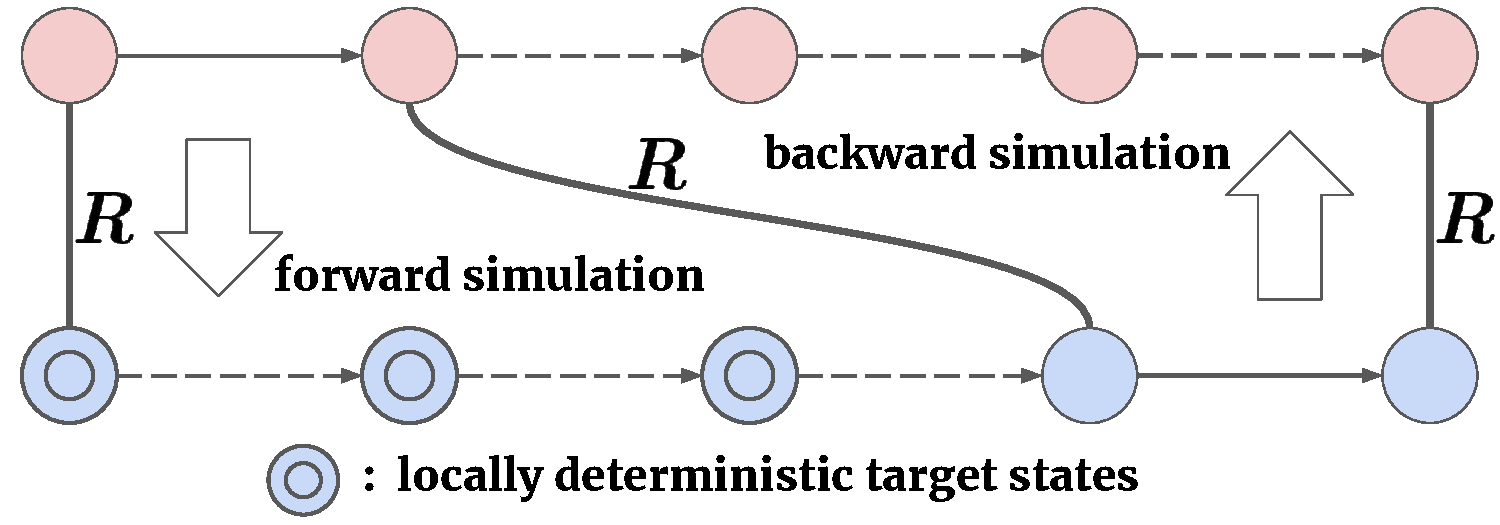
\includegraphics[width=0.7\textwidth]{images/mixed-sim-bold.pdf}
%% 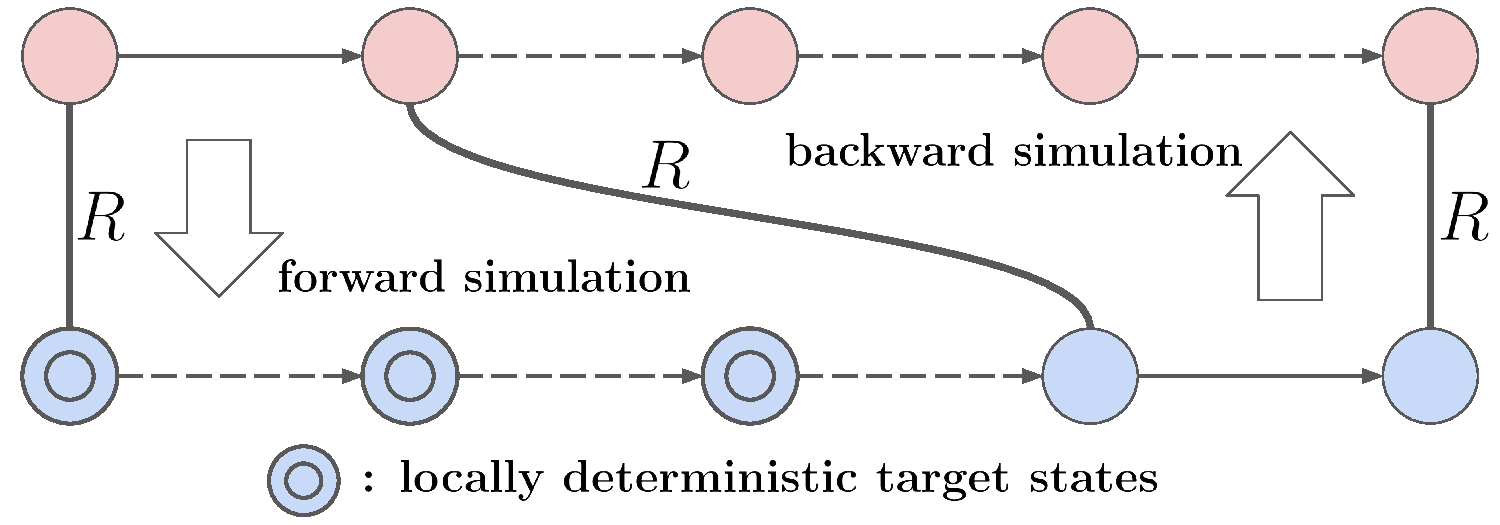
\includegraphics[width=0.7\textwidth]{images/mixed-sim.pdf}
\caption{A visualized example of mixed simulations}
\label{fig:mixedsim}
\end{figure}

\section{CompCertM}
\label{sec:compiler:compcertm}

Based on the theories we presented so far, we develop \ccm{}, an extension of \cc{} with the
repaired interaction semantics and open simulations to support multi-language linking.  We state
\ccm{}'s compositional correctness results (\Cref{sec:results:compiler}) and evaluate its
verification efforts (\Cref{sec:results:evaluation}).  \ccm{} currently supports the x86 backend only.
We do not currently see any technical problem with supporting other architectures.

\subsection{Compositional Correctness}
\label{sec:results:compiler}

\ccm{} uses open simulations with three parameters:
memory relations, symbol relations and memory predicates
(see \Cref{sec:main-verification:opensim} for details).
It supports $(i)$ the memory relations discussed in \Cref{sec:overview-verification:injection}:
identity, extension and (enriched) injections with no or any given module-local invariant;
$(ii)$ two symbol relations: one for keeping identical symbols in the source and target
and the other for allowing elimination of global variables in the target (only allowed for memory injections), needed for \code{Unusedglob} and \code{Unreadglob};
$(iii)$ two memory predicates: one for no analysis and the other for the value analysis of \cc{}.

Let $\rels$ be the set of open simulations with all possible parameters.
To apply RUSC, we prove that the \ccm{} compiler $\mathcal{C}$ transforms the source module with
a series of passes that are independently verified using open simulations in $\rels$.
\begin{lemma}[Pass Correctness]\label{thm:results-passes}
  For any \textrm{Clight} module $S$ and \textrm{Asm} module $T$, if $\mathcal{C}(S) = T$, then
  there exist intermediate modules $M_0, M_1, \cdots, M_n$ such that:
  \begin{enumerate}
  \item $M_0 = S$ and $M_n = T$; and
  \item $\forall i \in [0,n),~ \exists R \in \rels,~ (M_i, M_{i+1}) \in R$~.
  \end{enumerate}
\end{lemma}

We also prove all \textrm{Clight} and \textrm{Asm} modules are self-related.
\begin{lemma}[Self-Relatedness]\label{thm:results-relatedness} For any \textrm{Clight} or \textrm{Asm}
  module $M$, we have $M \in \self{\rels}$.
\end{lemma}
\noindent
\revision{Note that
  since we define illegal interference from Asm
  (\ie causing different behaviors in the source and target) as undefined behaviors (UBs)
  as shown in \Cref{sec:compiler:solution},
  every Asm module can be self-related.}

From \Cref{thm:results-passes,thm:results-relatedness}, the RUSC relation for the compiler follows.
\begin{theorem} [Modular Correctness]\label{thm:results-modular}
  For any \textrm{Clight} module $S$ and \textrm{Asm} module $T$, if $\mathcal{C}(S) = T$:
  \[
    {S} \rusc_\rels {T} \quad\text{with}\quad S,T \in \self{\rels}~.
  \]
\end{theorem}

\noindent
This theorem provides a truly compositional correctness
thanks to the compositionality of RUSC (\Cref{thm:rusc}):
%% The fact that the source and target are related by RUSC
%% implies that they satisfy behavioral refinement by adequacy of RUSC, and moreover
the relation can be freely (\ie vertically or horizontally) composed with any verification using RUSC
including that against mathematical specifications.
As an example, the following compositional correctness follows.
\begin{corollary} [Compositional Correctness 1]\label{thm:results-compiler}
  Let $(S_1,T_1), \ldots, (S_n,T_n)$ be pairs of source and target modules.
  If each pair is either compiled (\ie $\mathcal{C}(S_i) = T_i$ with $S_i$ \textrm{Clight} and $T_i$ \textrm{Asm}), or a self-related context (\ie $S_i = T_i \in \self{\rels}$), then
  \[
    \beh{S_1 \llink \cdots \llink S_n} \supseteq \beh{T_1 \llink \cdots \llink T_n}~.
  \]
\end{corollary}
%
\noindent This correctness theorem is compositional in the sense that behavior is refined in the
presence of any self-related contexts such as arbitrary \textrm{Clight} and \textrm{Asm} modules
(\Cref{thm:results-relatedness}).





Note that \textrm{Clight}, not \textrm{\cc{} C}, is the source language in the above theorems.  One of the
reasons is that \textrm{Clight} is the source language for most verification frameworks based on
\cc{}, such as VST~\cite{VST}, \ccc{}, and \ccx{}.  More importantly, we found that
\textrm{\cc{} C} is incompatible with memory injections.  Specifically,
\textrm{\cc{} C} imposes a strict alignment requirement on memory blocks of size zero, which, however,
%% but the requirement
is not preserved by memory injections.
%% For this reason, we cannot achieve full horizontal compositionality
%% in the presence of both \textrm{\cc{} C} modules and compiler passes verified using memory injections.
In other words, \textrm{\cc{} C} modules are not always self-related by memory injections.\footnote{This problem
  would be solved if one strengthens memory injections with more strict alignment requirements.}

\myparagraph{Supporting \textrm{\cc{} C}}
However, we can still prove a compositional correctness (not modular correctness as in \Cref{thm:results-modular}) for \textrm{\cc{} C}
following \scc{}'s \emph{Level A} technique~\cite{kang:scc},
which exploits the fact that all \textrm{CompCert C} modules are transformed to \textrm{Clight} modules
by the same two passes.
Specifically, the first pass is verified using an open simulation with the memory identity
and the second pass with memory injections, as done in the original \cc{}.
Then the following lemma follows from horizontal compositionality and adequacy of
open simulations (with memory identity and injection) and transitivity of behavioral refinement.

\begin{lemma} [ClightGen Correctness]\label{thm:results-clightgen}
  Let $(S_1,T_1), \ldots, (S_n,T_n)$ be pairs of source and target modules.
  If each pair is either translated (\ie $\textrm{ClightGen}(S_i) = T_i$ with $S_i$ \textrm{\cc{} C} and $T_i$ \textrm{Clight}), or a self-related context (\ie $S_i = T_i \in \self{\rels}$), then
  \[
    \beh{S_1 \llink \cdots \llink S_n} \supseteq \beh{T_1 \llink \cdots \llink T_n}~.
  \]
\end{lemma}



By composing \Cref{thm:results-compiler}, \Cref{thm:results-clightgen} and \Cref{thm:results-relatedness}, we have the following theorem.
\begin{theorem} [Compositional Correctness 2]\label{thm:results-compiler2}
  Let $(S_1,T_1), \ldots, (S_n,T_n)$ be pairs of source and target modules.
  If each pair is either compiled (\ie $\mathcal{C}(S_i) = T_i$ with $S_i$ \textrm{\cc{} C} or \textrm{Clight} and $T_i$ \textrm{Asm}), or a self-related context (\ie $S_i = T_i \in \self{\rels}$), then
  \[
    \beh{S_1 \llink \cdots \llink S_n} \supseteq \beh{T_1 \llink \cdots \llink T_n}~.
  \]
\end{theorem}


\myparagraph{Adequacy w.r.t. Physical Semantics}


We show that the repaired interaction semantics is adequate w.r.t. the physical semantics of \cc{},
where the former uses the language-independent linking $\llink$ and the latter the syntactic linking $\plink$
concatenating modules of the same language.

We prove that the physical semantics refines the repaired interaction semantics for \textrm{Asm} modules
using a closed simulation of \cc{} with memory injections.
\begin{theorem}[Adequacy w.r.t. Assembly]\label{thm:results-adequacy-asm}
  Let $M_1, \cdots, M_n$ be \textrm{Asm} modules.  We have:
  \[   \beh{M_1 \llink \ldots \llink M_n} \supseteq  \beh{M_1 \plink \ldots \plink M_n} ~.\]
\end{theorem}
\noindent
\revision{This theorem allows us to carry verification results on the interaction semantics such as \Cref{thm:results-compiler2}
down to \cc{}'s Asm semantics with syntactic linking.}



Conversely, we prove that the repaired interaction semantics refines the physical semantics for \textrm{\cc{} C} modules
using a closed simulation of \cc{} with memory identity.
This result is useful because we want to allow separate compilation (of C modules) on the compiler side, and on the program verification side, we want to hide complexities from inter-module steps.
\begin{theorem}[Adequacy w.r.t C]\label{thm:results-adequacy-c}
  Let $M_1, \cdots, M_n$ be \textrm{\cc{} C} modules.  We have:
  \[  \beh{M_1 \plink \ldots \plink M_n} \supseteq \beh{M_1 \llink \ldots \llink M_n}  ~.\]
\end{theorem}


In some sense, the \Cref{thm:results-compiler2,thm:results-adequacy-asm,thm:results-adequacy-c} together forms a strong stress-test for a language-independent linking, and our results show strong evidence that our repaired interaction semantics is indeed adequate (in a literal sense).
Specifically, if one of the three desiderata is missing, it is trivial to find language-independent linking satisfying the others.
Without \Cref{thm:results-adequacy-asm}, one can define interaction semantics to always execute UB; then, the other theorems become trivial.
Without \Cref{thm:results-adequacy-c}, one can define the behavior of interaction semantics to an empty set.
Without \Cref{thm:results-compiler2}, one can define $\llink \defeq \plink$.

%% These results mean that the repaired interaction semantics does not give too few behaviors to assembly programs (e.g., missing physically observable behaviors), nor does it give too many behaviors to well-typed C programs (e.g., giving UB to them).


Interestingly, by composing \Cref{thm:results-compiler2,thm:results-adequacy-asm,thm:results-adequacy-c}, we obtain
the same separate compilation correctness result of \scc{}~\cite{kang:scc}:

\begin{corollary}[Separate Compilation Correctness]
  Let $S_1, \ldots, S_n$ be \textrm{\cc{} C} modules and $T_1, \ldots, T_n$ be \textrm{Asm} modules.
  If $\mathcal{C}(S_i) = T_i$ for each $i$, we have:
  \[
    \beh{S_1 \plink \cdots \plink S_n} \supseteq \beh{T_1 \plink \cdots \plink T_n}~.
  \]
\end{corollary}

\youngju{Just mention that \ccc{} does not satisfy upperbound, and explain it in appendix?}
\youngju{here? or appendix?: To this end, we have strengthened \cc{}'s type checker in a number of
  ways, ruling out trivially wrong (according to C standard) programs more than before.  We rule out
  (i) a program that contains an identifier that is not declared in the module (ii) ``return''
  (without value) statement used for non-void function (iii) ``return'' (with value) statement used
  for void function (iv) function arguments containing void type.  (v) has duplicate (function or
  global variable) identifiers (vi) A function argument with size bigger than INT\_MAX (\cc{}
  already aborts on such programs)}





\subsection{Evaluation of Verification Efforts}\label{sec:results:evaluation}

\begin{table}[t]
\footnotesize

\parbox{\linewidth}{
\caption{SLOC of \ccm{} and related works --- compared to its baseline \cc{}, respectively}
\begin{tabu}{@{}l@{\hspace{1.55pt}}|[1.25pt]@{\hspace{1.55pt}} c @{\hspace{1.55pt}}|@{\hspace{1.55pt}} c @{\hspace{1.55pt}}|@{\hspace{1.55pt}} c @{\hspace{1.55pt}}|[1.25pt]@{\hspace{1.55pt}} c @{\hspace{1.55pt}}|@{\hspace{1.55pt}} c @{\hspace{1.55pt}}|[1.25pt]@{\hspace{1.55pt}}}
Portion     & \shortstack{\cc{} \\ 3.5} & \ccr{} 3.5        & \ccm{} pack                                               & \shortstack{\cc{}\\ 2.1} & \ccc{} \\
\hline
Pass Proofs & 34,376    & 35,893 (+4.41\%)  & \newrevision{4,923(+14.32\%)}                                          & 21,215    & 52,140 (+145.77\%) \\
The Rest    & 85,617    & 87,965 (+2.74\%)  & \newrevision{25,558(+29.85\%)}  & 59,365    & 107,910 \hspace{.6mm} (+81.77\%) \\
Total       & 119,993   & 123,858 (+3.22\%) & \newrevision{30,481(+25.40\%)}                                         & 80,580    & 160,050 \hspace{.6mm} (+98.62\%) \\
\end{tabu}
\\
\begin{tabu}{@{}l@{\hspace{1.55pt}}|[1.25pt]@{\hspace{1.55pt}} c @{\hspace{1.55pt}}|@{\hspace{1.55pt}} c @{\hspace{1.55pt}}|[1.25pt]@{\hspace{1.55pt}}}
Portion     & \shortstack{\cc{} \\ 3.0} & \ccx{}             \\
\hline
Pass Proofs & 26,466    & 30,572 (+15.51\%)  \\
The Rest    & 82,312    & 121,532 (+47.65\%) \\
Total       & 108,778   & 152,104 (+39.83\%) \\
\end{tabu}
\label{table:evaluation-ours}
}

%% \parbox{\linewidth}{
%% \label{table:evaluation-ours}
%% }
    
\parbox{0.38\linewidth}{
\vspace{4mm}
\caption{\mbox{Breakdown of \ccm{} pack}}
\begin{tabu}{@{}l | l@{}}
Portion                          & SLOC                                                                                                     \\
\hline
\revision{Proofs about Intermodule Steps} & \newrevision{4,923}                                                                                                    \\
Interaction Semantics/Properties & 1,940                                                                                                    \\
Language Semantics/Properties    & 1,701                                                                                                    \\
Self Simulations                 & \newrevision{5,593}                                                                                                    \\
\cc{}  Metatheory Extension      & \newrevision{4,688}                                                                                                    \\
\ccm{} Metatheory                & \newrevision{7,656}                                                                                                    \\
Mixed Simulation                 & 1,090                                                                                                    \\
Adequacy w.r.t. Asm              & 2,890                                                                                                    \\
\end{tabu}
\label{table:evaluation-breakdown}
}
\hfill
\parbox{0.45\linewidth}{
\vspace{4mm}
\caption{SLOC of additional developments}
%% \begin{tabu}{@{}l @{\;} |[1.25pt] @{\;} r @{\;} | @{\;} r @{\;} | @{\;} r @{\;} | @{\;} r @{\;} | @{\;} r @{}}
%% Portion                          & \shortstack{\texttt{Unreadglob} \\ 3.5} & \shortstack{\texttt{Unreadglob} \\ pack} & \texttt{mutual-sum} & \texttt{utod} & \shortstack{Adequacy \\ w.r.t. C} \\
%% \hline
%% Pass Proofs                      & 1,842                   & 338                      & 3,088               & 361           & -             \\
%% The Rest                         & 260                     & 1,933                    & 2,707               & 424           & 4,044         \\
%% Total                            & 2,102                   & 2,271                    & 5,795               & 785           & 4,044         \\
%% \end{tabu}
\begin{tabu}{@{}l @{\;} |[1.25pt] @{\;} r @{\;} | @{\;} r @{\;} | @{\;} r @{\;} | @{\;} r @{\;} | @{\;} r @{}}
Portion                          & \shortstack{\texttt{Unreadglob} \\ 3.5} & \shortstack{\texttt{Unreadglob} \\ pack} & \shortstack{Adequacy \\ w.r.t. C} \\
\hline
Pass Proofs                      & 1,842                   & 338                      & -             \\
The Rest                         & 260                     & 1,933                    & 4,044         \\
Total                            & 2,102                   & 2,271                    & 4,044         \\
\end{tabu}
\label{table:evaluation-others}
}%
\end{table}

\youngju{There are two ``unreadglob'' columns, one for \cc{} and one for pack. Simplify it}
\youngju{How about reducing caption text size?}
\jeehoon{``Per-pass'', ``Metatheory'', and ``Total'' instead of ``Pass Proofs'', ``The Rest'', and ``Whole''}

To demonstrate that \ccm{} is lightweight,
we compare significant lines of code (SLOC) of \ccm{}, \ccc{}, and \ccx{} with
those of their baseline \cc{} versions 3.5, 2.1, and 3.0, respectively.
Overall, \ccm{} adds less code to \cc{} than \ccc{} and \ccx{} do,
and in particular significantly less code than \ccc{} for the proofs of compiler passes.%
\footnote{\revision{Note that \ccc{} allows horizontal compositionality between any intermediate languages (ILs)
  while \ccm{} only between Clight and Asm since self-relatedness is proven only for the two.
  Though practically unnecessary, supporting linking between arbitrary ILs in \ccm{} would increase SLOC to prove self-relatedness for the other ILs.}}
\newrevision{Also note that \ccr{} uses the enriched memory injections of \Cref{sec:overview-verification:injection:dynamic} instead of the original memory injections
in order to give reusable main lemmas for both closed and open simulations.
Since \ccr{}'s pass proofs are only 4.41\% larger than \cc{}'s, 
the overhead due to handling the private memory components of enriched memory injections is, roughly speaking, at most 4.41\%.}

\Cref{table:evaluation-ours} summarizes the comparison.
For each compiler (\ie each column),
the rows report SLOC for the proofs of all compiler passes (Pass Proofs),
the rest of the development (The Rest),
and their summation (Total).
Note that \ccm{} is split into \ccr{} and \ccm{} pack, for which the former is our refactoring
of \cc{} and the latter is an additional package to support multi-language linking.
We counted SLOC reported by
\code{coqwc}.\footnote{Concretely, we counted ``spec'' and ``proof'' lines reported by \code{coqwc}.
  Because we use a different criteria for line numbers, they are different from those reported in
  prior work~\cite{stewart:ccc,gu:dscal,wang:saccx}.}  When counting SLOC, we excluded the following
code for fair comparison: $(i)$ code for other architectures than x86 because all three projects support
only x86; $(ii)$ code for the parser and type checker introduced in later versions of \cc{}; and $(iii)$ code for \textrm{ClightGen}, which is not supported by both \ccx{} and
\ccc{}.  We also excluded \ccc{}'s legacy proofs for the original compiler correctness.  We used the
latest development branches for the three projects.\footnote{Development as of November 8, 2019, available at: \url{https://github.com/snu-sf/compcertr}, \url{https://github.com/snu-sf/compcertm}, \url{https://github.com/PrincetonUniversity/compcomp}, \url{https://github.com/DeepSpec/dsss17/tree/master/CAL}}








\Cref{table:evaluation-breakdown} analyzes the \newrevision{30,481} SLOC for \ccm{} pack.
\revision{The pass proofs consist of \newrevision{4,923} SLOC for reasoning about intermodule steps, which is
  sometimes nontrivial since they perform the logical instrumentation presented in \Cref{sec:compiler:solution}.
  Note that \ccr{} provides proofs for intramodule steps as main lemmas, which are reused in \ccm{}.
}
The rest consists of
1,940 SLOC for the repaired interaction semantics and its properties;
1,701 SLOC for properties of each language such as determinism and receptiveness;
5,576 SLOC for self-relatedness (\Cref{thm:results-relatedness});
4,687 SLOC for extending the metatheory of CompCert;
7,569 SLOC for open simulations and other metatheory for \ccm{};
1,090 SLOC for mixed simulation; and
2,890 SLOC for adequacy w.r.t. assembly (\Cref{thm:results-adequacy-asm}).

%% \Cref{table:evaluation-others} shows SLOC for the new optimization pass and the verification examples
%% given in the dissertation.  Note that \code{Unreadglob} 3.5 adds the optimization to \ccr{} proving closed simulation
%% and \code{Unreadglob} pack to \ccm{} proving open simulation, which reuses the proof of \code{Unreadglob} 3.5 for intramodule steps.
%% As the verification of \code{mutual-sum} and \code{utod} show, directly proving
%% open simulation between programs and specifications is costly. 
%% We believe that program logics like VST~\cite{VST} can be used to prove such simulation,
%% which could significantly reduce the verification cost.
\Cref{table:evaluation-others} shows SLOC for the new optimization pass.  Note that \code{Unreadglob} 3.5 adds the optimization to \ccr{} proving closed simulation
and \code{Unreadglob} pack to \ccm{} proving open simulation, which reuses the proof of \code{Unreadglob} 3.5 for intramodule steps.


\section{Formal Semantics}
\label{sec:compiler:semantics}
abc

\section{Formalization of Verification Techniques}
\label{sec:compiler:verification}
abc

\section{Related Work}
\label{sec:compiler:related}
abc


\chapter{Application: Program Verification}
\label{chap:program}
\chapter{\;\;\;\;Program Verification}
\label{sec:program}

\section{Background}
\label{sec:program:background}

\section{Problems}
\label{sec:program:problems}

\section{Solution}
\label{sec:program:solution}


\chapter{Conculsion}
\label{chap:concl}
\input{concl}

%% \appendix

\chapter{My Appendix}
\lipsum[1-3]

\begin{thebibliography}{00}
\addcontentsline{toc}{chapter}{\bibname}

% 영문저널의 경우
    \bibitem{ref1} B. Jeon and J. Jeong, ``Blocking artifacts
    reduction in image compression with block boundary discontiunity
    criterion,'' {\em IEEE Transactions on Circuits and Systems for
    Video Tech.}, vol. 8, no.3, pp. 345-357, June 1998.

% 영문학술대회의 경우
    \bibitem{ref2} W. G. Jeon and Y. S. Cho, ``An equalization
    technique for OFDM and MC-CDMA in a multipath fading channels,''
    in {\em Proceedings of IEEE Conference on Acoustics, Speech and
    Signal Processing}, Munich, Germany, May 1997. pp. 2529-2532.

% 국내저널의 경우
    \bibitem{ref3} 김남훈, 정영철, ``평탄한 통과대역 특성을 갖는
    새로운 구조의 광도 파로열 격자 라우터,'' {\em 전자공학회논문지},
    제35권 D편, 제3호, 56-62쪽, 1998년 3월.

% 국내학술대회의 경우
    \bibitem{ref4} 윤남국, 김수종, ``무선 센서 네트워크에서의 에너지
    효율적인 그라디언트 기반 라우팅 기법,'' {\em 한국정보과학회
    2006년 추계학술대회}, 제12권, 제2호, 2006년 10월. pp.
    1372-1374.

% 단행본의 경우
    \bibitem{ref5} C. Mead and L. Conway, {\em Introduction to VLSI
    Systems}, Addison-Wesley, Boston, 1994.

% URL
    \bibitem{ref6} The SolarMESH Network,
    http://owl.mcmater.ca/solarmesh

% Technical Report의 경우
    \bibitem{ref7} K. E. Elliott and C. M. Greene, ``A local adaptive
    protocol,'' Argonne National Laboratory, Argonne, France,
    Technical Report 916-1010-BB, 1997.

% 학위논문의 경우
    \bibitem{ref8} T. Kim, ``Scheduling and Allocation Problems in
    High-level Synthesis,'' Ph. D. Dissertation, ECE Department,
    Univ. of Illinois at U-C, 1993.

% 특허의 경우
    \bibitem{ref9} Sunghyun Choi, ``Wireless MAC protocol based on a
    hybrid combination of slot allocation, token passing, and
    polling for isochronous traffic,'' U.S. Patent No. 6,795,418,
    September 21, 2004.

% 표준
    \bibitem{ref10} IEEE Std. 802.11-1999, Part 11: Wireless LAN
    Medium Access Control (MAC) and Physical Layer (PHY)
    specifications, Reference number ISO/IEC 8802-11:1999(E), IEEE
    Std. 802.11, 1999 edition, 1999.

\end{thebibliography}

\keywordalt{서울대학교, 전기공학부, 졸업논문}
\begin{abstractalt}
서울대학교 전기공학부 졸업논문 예제 파일입니다.
서울대학교 전기공학부 졸업논문 예제 파일입니다.
서울대학교 전기공학부 졸업논문 예제 파일입니다.
서울대학교 전기공학부 졸업논문 예제 파일입니다.
서울대학교 전기공학부 졸업논문 예제 파일입니다.
서울대학교 전기공학부 졸업논문 예제 파일입니다.
서울대학교 전기공학부 졸업논문 예제 파일입니다.
서울대학교 전기공학부 졸업논문 예제 파일입니다.
서울대학교 전기공학부 졸업논문 예제 파일입니다.
서울대학교 전기공학부 졸업논문 예제 파일입니다.

서울대학교 전기공학부 졸업논문 예제 파일입니다.
서울대학교 전기공학부 졸업논문 예제 파일입니다.
서울대학교 전기공학부 졸업논문 예제 파일입니다.
서울대학교 전기공학부 졸업논문 예제 파일입니다.
서울대학교 전기공학부 졸업논문 예제 파일입니다.
서울대학교 전기공학부 졸업논문 예제 파일입니다.
서울대학교 전기공학부 졸업논문 예제 파일입니다.
서울대학교 전기공학부 졸업논문 예제 파일입니다.
서울대학교 전기공학부 졸업논문 예제 파일입니다.
서울대학교 전기공학부 졸업논문 예제 파일입니다.
서울대학교 전기공학부 졸업논문 예제 파일입니다.
서울대학교 전기공학부 졸업논문 예제 파일입니다.
서울대학교 전기공학부 졸업논문 예제 파일입니다.
서울대학교 전기공학부 졸업논문 예제 파일입니다.
서울대학교 전기공학부 졸업논문 예제 파일입니다.
서울대학교 전기공학부 졸업논문 예제 파일입니다.
\end{abstractalt}

\acknowledgement
Thanks!

\end{document}

